\chapter{El caso finito}
\noindent
Inspirados por el teorema \ref{theory:th:feasibility}, en este capítulo analizamos el
caso en el que el vector coprimo $\vec{q}$ tiene entradas estrictamente positivas. De esta manera,
el problema \eqref{theory:formulation} deviene una instancia particular del famoso Problema de la
Mochila:
\begin{subequations}
	\label{knapsack-formulation}
	\begin{align}
		\max_{\vec{x} \in \Z^n} \quad
			& \vec{u}^T\vec{x}, \\
		\text{s.a.} \quad
			& \vec{w}^T\vec{x} \leq u, \\
			& \vec{x} \geq \vec{0},
	\end{align}
\end{subequations}
donde los vectores positivos $\vec{u}, \vec{w} \in \Z^n$ son conocidos como
vector de útiles y vector de pesos, respectivamente. Puesto que no acotamos
$\vec{x}$, el problema recibe el nombre de Problema de la Mochila no Acotado.
Analizaremos el caso $\vec{u} = \vec{w}$, el cual es es considerado como un
Problema de la Suma de Conjuntos no Acotado.

En la primera sección realizamos un análisis de capas enteras a fin de obtener
un resultado análogo al teorema \ref{infinite:th:complexity}. En concreto, el
teorema \ref{th:intnonneg2} enuncia que, para un presupuesto $u$
suficientemente grande en el problema \eqref{theory:formulation}, la búsqueda
de una solución se reduce a resolver solamente una ecuación lineal diofantina.

El resultado anterior, si bien es interesante, solo es de existencia y no
muestra cómo obtener las soluciones enteras no negativas de ecuaciones lineales
diofantinas. De manera similar a como lo hicimos en el capítulo anterior, la
segunda sección se encarga de presentar la construcción de soluciones a partir
de los algoritmos \ref{algo:fin:helper} (pág.~ \pageref{algo:fin:helper}) y
\ref{algo:fin:dioph} (pág.~ \pageref{algo:fin:dioph}).

Finalmente, en la tercera y última sección de este capítulo, realizamos algunos experimentos
numéricos que comparan la eficacia de nuestros algoritmos recién desarrollados con la de
Ramificación y Acotamiento, así como de una formulación alternativa de programación dinámica.

\section{Análisis de capas enteras}
\noindent
De acuerdo al segundo caso del teorema \ref{theory:th:feasibility}, el número de puntos enteros no
negativos sobre la $k$-ésima capa entera es finito y, por lo tanto, puede ser cero. Sea $k \in
\braces{\eta, \eta - 1, \ldots, 0}$. Sabemos de la sección \ref{subsec:dioph-eq} que deseamos resolver la
ecuación lineal diofantina \eqref{eq:dioph}, por lo que implementamos la misma estrategia para
plantear una formulación recursiva. 

Debido al supuesto $\vec{q} > \vec{0}$, observemos de \eqref{dummy:eq:ith-equation} que podemos
agregar la condición $\omega_{i} \geq 0$, en efecto, buscamos que $\vec{x}$ sea no negativo y
recordemos que $g_i$ es un máximo común divisor (ver \eqref{dummy:eq:ith-g}), por lo que es
estrictamente positivo. Juntando esto con el supuesto $\vec{q} > \vec{0}$, encontramos que
$\omega_i$ es no negativo para toda $i \in \braces{1, \ldots, n - 1}$. Así pues, despejando $t_i$ de
\eqref{eq:recurrence} obtenemos los intervalos de factibilidad
\begin{equation*}
	\label{phase-1:finite:eq:param-bounds}
	\left\lceil -\frac{\omega_ix_i'}{g_{i+1}} \right\rceil
	\leq
	t_i
	\leq
	\left\lfloor \frac{\omega_i\omega_{i+1}'}{q_i} \prod_{j=1}^{i}g_j \right\rfloor,
\end{equation*}
para todo $i \in \lbrace 1, \ldots, n - 2\rbrace$. Luego, como $0 < q_{n - 1}, q_n$, se sigue de
\eqref{eq:last-solution} que
\begin{equation*}
	\label{phase-1:finite:eq:param-bounds-last}
	\left\lceil -\frac{\omega_{n-1}x_{n-1}'}{q_n} \cdot \prod_{j=1}^{n-1}g_j \right\rceil
	\leq
	t_{n - 1}
	\leq
	\left\lfloor \frac{\omega_{n-1}x_{n}'}{q_{n-1}} \cdot \prod_{j=1}^{n-1}g_j \right\rfloor.
\end{equation*}

Consecuentemente, el número de elecciones que podemos realizar para el vector
de variables libres $\vec{t} \in \Z^{n-1}$ es finito, como lo confirma el
teorema \ref{theory:th:feasibility}. Si determinamos que no existe tal punto
$\vec{t}$ en la $k$-ésima capa entera, descendemos a la $(k -1)$-ésima capa
entera y continuamos con nuestra búsqueda.

% Observemos también que una elección de $t_i$ modifica $\omega_{i+1}$ y por lo tanto también afecta
% el intervalo de factibilidad de $t_{i+1}$. Siguiendo con este razonamiento, encontramos que una
% elección de $t_i$ afecta a su vez los intervalos de factibilidad de $t_{i+1}, \ldots, t_{n-1}$. En
% la sección \ref{subsec:complex} discutiremos cómo es que esta ``cadena'' acota la complejidad
% algorítmica del algoritmo \ref{algo:fin:dioph}.

Ahora bien, en esta primera parte de la sección nos encargamos de calcular una cota superior para el
número de capas enteras que debemos analizar de manera que garanticemos la existencia de un punto
entero no negativo sobre una de estas capas enteras.

% En la primera parte de esta sección determinamos una cota superior para el número de capas enteras
% que visitamos y analizamos el comportamiento a medida que el presupuesto $u$ aumenta. En la segunda
% parte de esta sección mostramos que si el presupuesto $u$ es suficientemente grande, entonces la
% solución de (\ref{theory:formulation}) sí se encuentra sobre la $\eta$-ésima capa entera. Este
% resultado es análogo al caso infinito del teorema \ref{theory:th:feasibility}. Finalmente, en la
% tercera parte de esta sección discutimos brevemente sobre la complejidad algorítmica de encontrar
% la solución.

\begin{lemma}
	\label{lemma:tau}
	Sea $\vec{p} \in \R^n$ un vector esencialmente entero y sea $\vec{q} \in \Z^n$ su múltiplo
	coprimo, por lo que existe $m \in \R$ tal que $\vec{p} = m\vec{q}$. Supongamos que $m > 0$ y que
	$\vec{q} > \vec{0}$. Sea $q^* \coloneq \max\lbrace q_1, \ldots, q_n \rbrace$, y sea
	\begin{equation}
		\label{eq:tau}
		\tau \coloneq \left\lfloor \left\lfloor \frac{u}{q^*} \right\rfloor
			\frac{q^*}{m} \right\rfloor,
	\end{equation}
	donde $u$ es el lado derecho de \eqref{theory:constraint:budget}. Entonces la solución del
	problema \eqref{theory:formulation}, de ser factible, se encuentra en una capa entera
	parametrizada por $k \in \lbrace \eta, \eta - 1, \ldots, \tau \rbrace$, donde recuperamos $\eta$
	del lema \ref{phase-1:lemma:eta}.
\end{lemma}
\begin{proof}
	Definamos $i^* \coloneq \argmax\braces{q_1, \ldots, q_n}$ y consideremos el vector
	\begin{equation*}
		\vec{v} \coloneq \left\lfloor \frac{u}{q^*} \right\rfloor \vec{e}_{i^*}.
	\end{equation*}
	Por hipótesis tenemos $q^* > 0$ y, además, como el problema
	\eqref{theory:formulation} es factible, se sigue del teorema \ref{theory:th:feasibility} que el
	presupuesto $u$ es no negativo. De esto obtenemos que $\vec{v} \geq \vec{0}$. Así también,
	\begin{equation*}
		\vec{q}^T\vec{v} = \left\lfloor \frac{u}{q^*} \right\rfloor q^*
		\leq \frac{u}{q^*}q^* = u,
	\end{equation*}
	y entonces $\vec{v}$ es factible. De aquí se sigue que este vector provee
	una cota inferior para valor óptimo del problema
	(\ref{theory:formulation}). Así pues, todo vector $\vec{x}$ candidato a ser
	el óptimo del problema satisface
	\begin{equation*}
		\vec{q}^T\vec{x} = \frac{\vec{p}^T\vec{x}}{m} \geq \frac{\vec{q}^T\vec{v}}{m} = 
		\floor{\frac{u}{q^*}} \frac{q^*}{m}.
	\end{equation*}
	Nos interesa determinar el entero $\tau$ más pequeño tal que todo punto sobre la capa
	entera $H_{\vec{q}, k\norm{\vec{q}}^{-2}}$ con $k \in \lbrace \tau, \tau + 1, \ldots \rbrace$
	satisfaga esta desigualdad. Del lema \ref{phase-1:lemma:layer}, encontramos que $k$ debe satisfacer
	\begin{equation*}
		\frac{k}{\norm{\vec{q}}^{2}} = \frac{\vec{q}^T\vec{x}}{\norm{\vec{q}}^2} \geq
		\left\lfloor \frac{u}{q^*} \right\rfloor \frac{q^*}{m}
		\frac{1}{\norm{\vec{q}}^2},
	\end{equation*}
	equivalentemente,
	\begin{equation*}
		k \geq \floor{\frac{u}{q^*}}\frac{q^*}{m}.
	\end{equation*}
	Consecuentemente,
	\begin{equation*}
		\tau =
		\left\lfloor \left\lfloor \frac{u}{q^*} \right\rfloor \frac{q^*}{m}
			\right\rfloor.
	\end{equation*}
	Finalmente, recordemos del lema \ref{phase-1:lemma:eta} que $\eta$ es la primera capa en
	satisfacer la restricción presupuestaria. Por lo tanto, el óptimo del problema
	\eqref{theory:formulation} se encuentra en una capa entera parametrizada por $\tau \leq k \leq \eta$.
\end{proof}

\begin{observation}
	Siempre se cumple que $\tau \leq \eta$. En efecto,
	\begin{equation*}
		\left\lfloor \frac{u}{q^*} \right\rfloor q^*
		\leq \frac{u}{q^*} q^* = u,
	\end{equation*}
	como $m > 0$, tenemos
	\begin{equation*}
		\left\lfloor \frac{u}{q^*} \right\rfloor \frac{q^*}{m}
		\leq \frac{u}{m}.
	\end{equation*}
	Aplicando la función piso a ambos lados de la desigualdad y comparando con \eqref{eq:tau} y el
	lema \ref{phase-1:lemma:eta} encontramos que $\tau \leq \eta$.
\end{observation}
\begin{observation}
	Nuevamente, la suposición de que el escalar $m$ sea positivo ocurre sin pérdida de generalidad.
	Así como mencionamos en el capítulo anterior que si $m$ es negativo entonces existe un parámetro
	$\eta'$ análogo a $\eta$, también existe $\tau' \geq \eta'$ tal que la solución del problema
	\eqref{theory:formulation} se encuentra en una capa parametrizada por $\eta' \leq k \leq \tau'$.
\end{observation}


% Es decir, a pesar de que el óptimo se encuentre sobre la capa entera $k$ que estamos analizando, la
% elección de los primeros parámetros que realicemos puede afectar el tiempo de terminación de nuestro
% algoritmo. Hay dos extremos en las posibles estrategias que podemos adoptar para realizar estas
% elecciones. Para visualizarlo, tenemos que nuestro presupuesto actual $\omega_{i}$ determina el
% siguiente presupuesto a partir de
% \begin{equation*}
% 	\begin{cases}
% 		x_i = \omega_ix_i' + g_{i+1}t_i, \\
% 		\omega_{i+1} = \omega_i\omega_{i+1}' - \frac{q_i}{\prod_{j=1}^{i}g_j}t_i,
% 	\end{cases}
% \end{equation*}
% donde la primera ecuación indica cuántos elementos de $x_i$ decidimos adquirir a partir del
% presupuesto actual $\omega_i$.
% 
% El primer extremo está en buscar agotar todo nuestro presupuesto disponible en las primeras
% elecciones de $x_1, x_2, \ldots, x_i$. Es decir, adquirimos la mayor cantidad que
% podamos de los primeros productos. Bajo esta perspectiva, es razonable imponer un orden en $\vec{q}$
% de manera que
% \begin{equation*}
% 	q_1 \geq q_2 \geq \cdots \geq q_n,
% \end{equation*}
% por lo que primero adquirimos los artículos más caros. En este caso diremos que $\vec{q}$ está en
% orden descendente. Si adoptamos esta estrategia es porque suponemos que el óptimo se concentra en
% una vecindad de los primeros $i$ artículos. Es decir, si tenemos la creencia de que $x_{i +
% 1}, \ldots, x_n$ pueden ser aproximadamente cero.
% 
% % TODO: es mejor argumentar esto en la sección de análisis de resultados.
% % De ser este el caso, entonces es razonable suponer que los tiempos de terminación de esta búsqueda
% % son similares a los de Ramificación y Acotamiento. 
% 
% El segundo extremo es esencialmente lo opuesto. Esto no quiere decir que ahora ordenamos $\vec{q}$
% de manera ascendente y escogemos las primera $t_i$ lo más pequeñas posible\footnote{Si
% 	hiciéramos esto es porque creemos que $x_1, \ldots, x_i$ son aproximadamente cero,
% 	pero entonces podemos permutar estas entradas de manera que se encuentren hasta el final y
% emplear la primera estrategia.}. Consiste en escoger $t_i$ de manera que se encuentre en el
% punto medio de sus cotas inferiores y superiores. Es decir, creemos que el óptimo se encuentra en
% una vecindad del centro de masa de la $k$-ésima capa entera.
% 
% Observemos que, independientemente del caso, si una capa entera no contiene puntos factibles,
% entonces ambas estrategias agotan todas las elecciones posibles de $t_1, \ldots,
% t_{n-1}$. Por lo tanto, los tiempos de terminación de ambas estrategias son iguales para capas
% enteras que no contienen puntos óptimos. La segunda estrategia, no obstante, es candidata ideal para
% realizar una búsqueda binaria. Discutimos más sobre esto último en la sección de análisis de
% resultados.

\begin{lemma}
	\label{lemma:layer-dist}
	Sean $q$ y $m$ enteros distintos de cero. Entonces la función $\Delta \colon \R \to \R$ dada por
	\begin{align*}
		\Delta(x) &\coloneq \left\lfloor \frac{x}{m} \right\rfloor - \left\lfloor \left\lfloor
		\frac{x}{q} \right\rfloor \frac{q}{m} \right\rfloor,
	\end{align*}
	es periódica con periodo $\lcm{q, m}$.
\end{lemma}
\begin{proof}
	Tenemos
	\begin{align*}
		\Delta(x + \lcm{q, m})
		&= \left\lfloor \frac{x}{m} + \frac{\lcm{q, m}}{m} \right\rfloor
		- \left\lfloor \left\lfloor \frac{x}{q} + \frac{\lcm{q,m}}{q} \right\rfloor \frac{q}{m}
			\right\rfloor,
	\end{align*}
	pero $q, m \mid \lcm{q, m}$, por lo que $\lcm{q,m}/m$ y $\lcm{q,m}/q$ son enteros. Por las
	propiedades de la función piso obtenemos:
	\begin{align*}
		\Delta(x + \lcm{q,m})
		&=
		\left\lfloor \frac{x}{m} \right\rfloor + \frac{\lcm{q,m}}{m}
		- \left\lfloor \left\lfloor \frac{x}{q} \right\rfloor\frac{q}{m} + 
			\frac{\lcm{q,m}}{q}\cdot\frac{q}{m} \right\rfloor \\
		&= 
		\left\lfloor \frac{x}{m} \right\rfloor + \frac{\lcm{q,m}}{m}
		- \left\lfloor \left\lfloor \frac{x}{q} \right\rfloor\frac{q}{m}\right\rfloor
		- \frac{\lcm{q,m}}{m} \\
		&= 
		\left\lfloor \frac{x}{m} \right\rfloor
		- \left\lfloor \left\lfloor \frac{x}{q} \right\rfloor\frac{q}{m}\right\rfloor \\
		&= \Delta(x),
	\end{align*}
	que es lo que queríamos demostrar.
\end{proof}
\begin{definition}
	Sea $\vec{p} \in \R^n$ un vector esencialmente entero y sea $\vec{q} \in \Z^n$ su múltiplo
	coprimo. Consideremos los parámetros $\eta$ y $\tau$ (c.f. lemas \ref{phase-1:lemma:eta} y
	\ref{lemma:tau}) como funciones del presupuesto $u$. Entonces decimos que la función $\Delta^*
	\colon \R \to \R$ dada por
	\begin{equation}
		\label{eq:dist-layers}
		\Delta^*(u) \coloneq \eta(u) - \tau(u)
	\end{equation}
	denota el \textbf{número de capas enteras a revisar} dado el presupuesto $u$.
\end{definition}

Si queremos aplicar el lema \ref{lemma:layer-dist} a la función de la definición anterior, debemos
reducir nuestra atención a vectores $\vec{p}$ enteros. Esto se debe a que debemos asegurar que el
múltiplo $m$ sea entero\footnote{
	Es la creencia del autor que el lema \ref{lemma:layer-dist} puede ser generalizado para
	$m$ racional.
}. Independientemente del comportamiento
periódico de $\Delta^*$, tenemos que esta función varía significativamente ante cambios en $m$.
Esto último implica que el número de capas enteras a revisar depende del número de cifras decimales
usadas para especificar $\vec{p}$.

\begin{example}
	\label{ex:decimals}
	Si tenemos $\vec{p} \coloneq (9.6, 7.2, 5.6)^T$, entonces $m = 0.8$ y por lo tanto el número de
	capas a revisar dado $u \coloneq 119$ es $\Delta^*(u) = 13$. En cambio, si tenemos $\vec{p} \coloneq
	(9.60, 7.28, 5.68)^T$, obtenemos $m = 0.08$, por lo que el número de capas a revisar dado $u$ es
	$\Delta^*(u) = 1487$. Eso ilustra la sensitividad de $\Delta^*$ con respecto a $m$.
\end{example}

% \begin{figure}[htbp]
%   \centering
% 
%   \begin{minipage}[t]{0.48\textwidth}
%     \centering
%     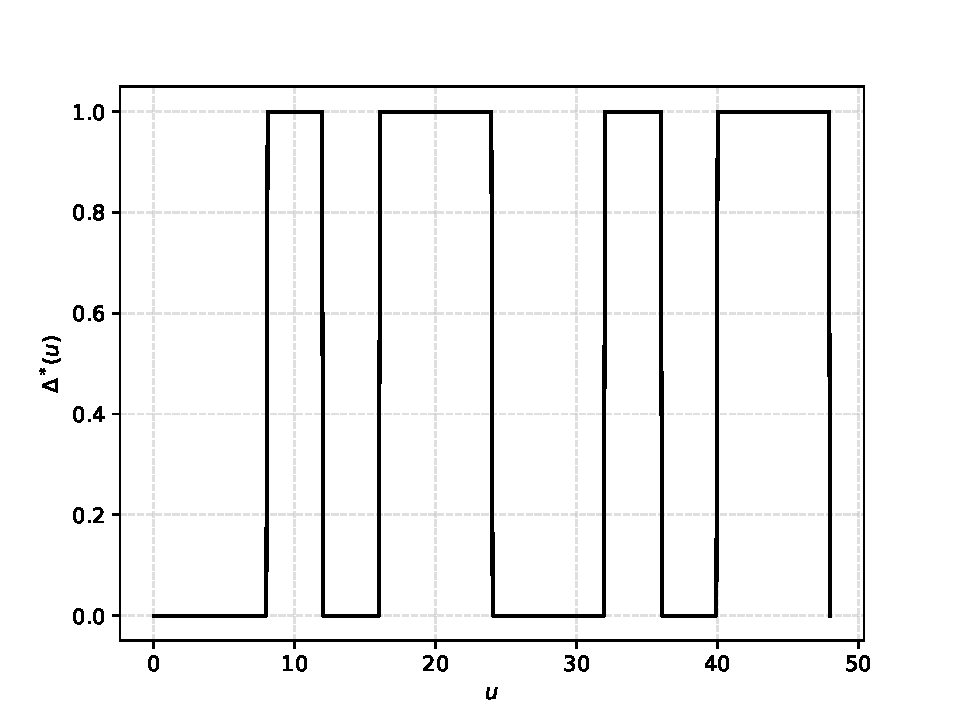
\includegraphics[width=\linewidth]{/home/tempdata/repos/thesis/static/misc/delta8m12q.pdf}
%   \end{minipage}
%   \hfill
%   \begin{minipage}[t]{0.48\textwidth}
%     \centering
%     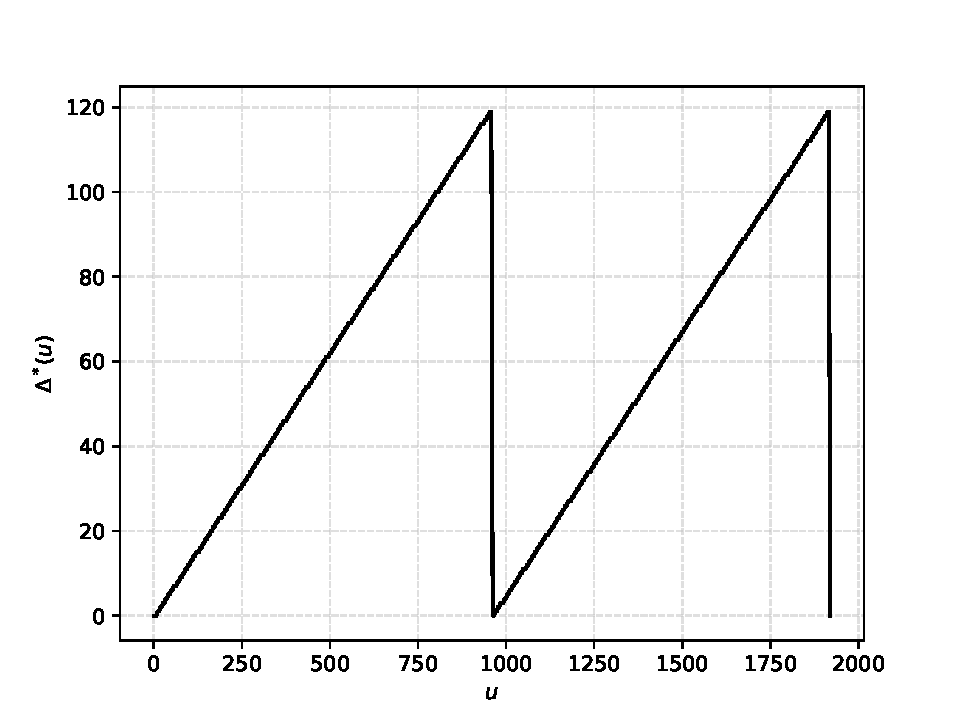
\includegraphics[width=\linewidth]{/home/tempdata/repos/thesis/static/misc/delta008m960q.pdf}
%   \end{minipage}
% 
%   \caption{Número de capas a revisar en función del presupuesto. \textit{Izquierda: }Para los
% 	  parámetros $m = 8$ y $q^* = 12$ encontramos que hay un máximo de una capa a revisar.
% 	\textit{Derecha: } A medida que $m$ se vuelve fraccionario, las capas a revisar aumentan. En
% 		este caso tenemos $m = 0.08$ y $q^* = 960$.}
%   \label{fig:m:ex}
% \end{figure}

% TODO: FIX (ver anotaciones de andreas)
% Observaremos en el análisis de resultados que el número de capas enteras que nuestro algoritmo
% revisa en realidad disminuye a medida que aumenta el presupuesto $u$.

En esta segunda parte de la sección, demostraremos que para un presupuesto $u$ suficientemente
grande, la solución del problema \eqref{theory:formulation} se encuentra en la $\eta$-ésima capa
entera donde, como siempre, $\eta$ es recuperada del lema \ref{phase-1:lemma:eta}. Este resultado
será análogo al teorema \ref{infinite:th:complexity}. No obstante, para lograr aquello, necesitamos
de un par de definiciones y lemas preliminares.

Para motivar al lector, primero mostramos que existe una vecindad fija de todo punto en $\R^n$ de
manera que esa vecindad contiene al menos un punto entero. Esto será especificado en el teorema
\ref{lemma:ball-cover}.

Luego, observamos que el ``trozo'' no negativo de una capa entera $H_{\vec{q},
k\norm{\vec{q}}^{-2}}$ crece a medida que $k$ aumenta. Recordemos que $k \leq
\eta$ y, por el lema \ref{phase-1:lemma:eta}, $\eta$ depende del lado derecho
$u$ de \eqref{theory:constraint:budget}. Así pues, si el presupuesto $u$ lo
permite, habrá un punto sobre ese trozo no negativo cuya vecindad también se
encuentra contenida en ese trozo y, por lo tanto, habrá un punto entero no
negativo sobre ese trozo. Esto será especificado en el teorema
\ref{th:intsimplex}.

Finalmente, relacionamos el punto entero que se encuentra sobre el pedazo no negativo de
$H_{\vec{q}, k\norm{\vec{q}}^{-2}}$ con el problema \eqref{theory:formulation}. Así pues, concluiremos
esta sección con los teoremas \ref{th:intnonneg1} y \ref{th:intnonneg2}.

\begin{definition}
	\label{fin:def:ball}
	Sea $\vec{q} \in \Z^n$ un vector coprimo y sea $k$ un entero. Entonces definimos la
	\textbf{bola cerrada} sobre la $k$-ésima capa entera $H_{\vec{q}, k\norm{\vec{q}}^{-2}}$ con
	radio $r > 0$ y centro $\vec{x} \in H_{\vec{q}, k\norm{\vec{q}}^{-2}}$ como
	\begin{equation}
		\label{eq:k-ball}
		B_r^{(k)}(\vec{x}) \coloneq \lbrace \vec{y} \in \R^n \colon \norm{\vec{y} - \vec{x}} \leq r
		\rbrace \cap H_{\vec{q}, k \norm{\vec{q}}^{-2}}.
	\end{equation}
\end{definition}
% TODO: mostrar una imagen con una bola.
\begin{theorem}
	\label{lemma:ball-cover}
	Sea $\vec{q} \in \Z^n$ un vector coprimo y supongamos que $q_n \neq 0$. Sea $k$ un entero.
	Entonces existe $r > 0$ tal que la familia de bolas
	\begin{equation*}
		\left\lbrace B_r^{(k)}(\vec{x}) \colon \vec{x} \in H_{\vec{q}, k\norm{\vec{q}}^{-2}} \cap
			\Z^n \right\rbrace
	\end{equation*}
	es una cubierta de la $k$-ésima capa entera $H_{\vec{q}, k\norm{\vec{q}}^{-2}}$.
\end{theorem}
\begin{proof}
	Como $q_n \neq 0$, recordemos del teorema \eqref{th:lattice} que
	\begin{equation*}
		\vec{x} \in H_{\vec{q}, k\norm{\vec{q}}^{-2}} \cap \Z^n \iff \vec{x} = k\vec{\nu} + M\vec{t}
	\end{equation*}
	para algún vector $\vec{t} \in \Z^{n-1}$, donde recuperamos $\vec{\nu}$ y $M$ de
	\eqref{eq:vec-omega} y \eqref{eq:mat-T}, respectivamente. Así, tenemos
	\begin{equation*}
		\left\lbrace B_r^{(k)}(\vec{x}) \colon \vec{x} \in H_{\vec{q}, k\norm{\vec{q}}^{-2}} \cap
			\Z^n \right\rbrace
			=
		\left\lbrace B_r^{(k)}(k\vec{\nu} + M\vec{t}) \colon \vec{t} \in \Z^{n-1} \right\rbrace.
	\end{equation*}
	Por la definición \ref{fin:def:ball} sabemos que $B_r^{(k)}(k\vec{\nu} + M\vec{t}) \subseteq H_{\vec{q},
	k\norm{\vec{q}}^{-2}}$ para todo $r > 0$ y para todo $\vec{t} \in \Z^{n-1}$. Luego, para
	cualquier $r > 0$ tenemos
	\begin{equation}
		\label{eq:ball-cover:1}
		\bigcup_{\vec{t} \in \Z^{n-1}}B_r^{(k)}(k\vec{\nu} + M\vec{t}) \subseteq
		H_{\vec{q}, k\norm{\vec{q}}^{-2}}.
	\end{equation}
	Ahora bien, sea $\vec{y}$ un punto sobre la $k$-ésima capa entera. Por el
	teorema \ref{th:lattice} sabemos que las columnas de $M$ son linealmente
	independientes, y entonces existe $\tvec{t} \in \R^{n-1}$ tal que
	\begin{equation*}
		\vec{y} = k\vec{\nu} + M\tvec{t}.
	\end{equation*}
	Sea $\vec{t} \in \Z^{n-1}$ el vector resultante de redondear cada entrada de
	$\vec{t}$ al entero más cercano. Luego, $\tvec{t} = \vec{t} + \vec{\delta}$,
	para alguna $\vec{\delta} \in \R^{n-1}$ que satisface $\norm{\vec{\delta}}_{\infty} \leq 1/2$.
	Definamos
	\begin{equation*}
		\vec{x} \coloneq k\vec{\nu} + M\vec{t} \in \Z^{n-1},
	\end{equation*}
	de donde se sigue que
	\begin{equation*}
		\norm{\vec{y} - \vec{x}}
		= \norm{M\vec{\delta}}
		\leq \norm{M}\norm{\vec{\delta}}
		\leq \sqrt{n - 1}\norm{M}\norm{\vec{\delta}}_\infty
		\leq \frac{\sqrt{n - 1}}{2}\norm{M}.
	\end{equation*}
	% \begin{align}
	% 	\norm{\vec{y} - \vec{x}}^{2} 
	% 	&= \norm{M\vec{\delta}}^{2} \nonumber \\
	% 	&\leq \sum_{i=1}^{n-1}|\delta_i|^2 \norm{M\vec{e}_i}^{2} \nonumber \\
	% 	&\leq \frac{1}{4}\sum_{i=1}^{n-1} \norm{M\vec{e}_i}^{2} \label{eq:alt-M-bound} \\
	% 	&= \frac{1}{4}\norm{M}_F^2, \nonumber
	% \end{align}
	% donde $\norm{M}_F$ denota la norma Frobenius de $M$.
	Por lo tanto, si definimos
	\begin{equation}
		\label{eq:radius}
		r \coloneq \frac{\sqrt{n - 1}}{2}\norm{M},
	\end{equation}
	encontramos que $\vec{y} \in B_r^{(k)}(\vec{x})$. Luego, como $\vec{y} \in H_{\vec{q},
	k\norm{\vec{q}}^2}$ fue genérico, tenemos que si $r$ está definido por \eqref{eq:radius},
	entonces
	\begin{equation}
		\label{eq:ball-cover:2}
		H_{\vec{q}, k\norm{\vec{q}}^{-2}} \subseteq
		\bigcup_{\vec{t} \in \Z^{n-1}}B_r^{(k)}(k\vec{\nu} + M\vec{t}).
	\end{equation}
	Juntando esto con (\ref{eq:ball-cover:1}) obtenemos lo que queríamos demostrar.
\end{proof}

Lo que se encuentra a continuación se encarga de formalizar y caracterizar lo
que nos referíamos anteriormente como ``trozo no negativo'' de la $k$-ésima
capa entera. Todas las definiciones fueron tomadas del capítulo 2 de
\cite{boyd} a excepción del baricentro, mientras que las demostraciones de los
lemas y teoremas fueron realizadas completamente por el autor.
\begin{definition}
	\label{def:aff}
	Sean $\vec{v}_1, \ldots, \vec{v}_m \in \R^n$ una colección de vectores,
	entonces definimos su \textbf{combinación afina} a partir de
	\begin{equation*}
		\aff\braces{\vec{v}_1, \ldots, \vec{v}_m} \coloneq \braces{\theta_1\vec{v}_1 + \cdots + \theta_m\vec{v}_m
		\colon \theta_1 + \cdots + \theta_m = 1}.
	\end{equation*}
\end{definition}

\begin{lemma}
	\label{lemma:aff}
	Sean $\vec{v}_1, \ldots, \vec{v}_m \in \R^n$ una colección de vectores. Entonces
	\begin{equation*}
		\aff\braces{\vec{v}_1, \ldots, \vec{v}_m} = \vec{v}_j + \gen\braces{\vec{v}_i -
		\vec{v}_j}_{i=1}^{n} = \vec{v}_j + \gen\braces{\vec{v}_i - \vec{v}_j}_{i\neq j}.
	\end{equation*}
\end{lemma}
\begin{proof}
	Puesto que $\vec{v}_j - \vec{v}_j = \vec{0}$, se sigue inmediatamente que
	\begin{equation*}
		\vec{v}_j + \gen\braces{\vec{v}_i - \vec{v}_j}_{i = 1}^{n}
		=
		\vec{v}_j + \gen\braces{\vec{v}_i - \vec{v}_j}_{i \neq j}.
	\end{equation*}
	Sean $\theta_1, \ldots, \theta_m$ escalares tales que $\theta_1 + \cdots + \theta_m = 1$. Por un
	lado, tenemos
	\begin{align*}
		\sum_{i=1}^{m}\theta_i\vec{v}_i
		&= \sum_{i=1}^{m}\theta_i\vec{v}_j + \sum_{i=1}^{m}\theta_i(\vec{v}_i - \vec{v}_j)  \\
		&= \vec{v}_j  + \sum_{i \neq j}\theta_i(\vec{v}_i - \vec{v}_j).
	\end{align*}
	De donde se sigue que $\aff\braces{\vec{v}_1, \ldots, \vec{v}_m} \subseteq \vec{v}_j +
	\gen\braces{\vec{v}_i - \vec{v}_j}_{i \neq j}$.

	Ahora bien, sea $\braces{\lambda_i}_{i \neq j}$ un conjunto de $m - 1$ escalares y definamos
	\begin{equation*}
		\lambda_j = 1 - \sum_{i \neq j}\lambda_i.
	\end{equation*}
	Observemos que $\lambda_1 + \cdots + \lambda_m = 1$ y, además,
	\begin{align*}
		\vec{v}_j + \sum_{i \neq j}\lambda_i(\vec{v}_i - \vec{v}_j)
		&= \left(1 - \sum_{i \neq j}\lambda_i\right)\vec{v}_j
		+ \sum_{i \neq j}\lambda_i\vec{v}_i \\
		&= \lambda_j\vec{v}_j + \sum_{i \neq j}\lambda_i\vec{v}_i \\
		&= \sum_{i = 1}^{m}\lambda_i\vec{v}_i.
	\end{align*}
	De donde se sigue que $\vec{v}_j + \gen\braces{\vec{v}_i - \vec{v}_j}_{i \neq j} \subseteq
	\aff\braces{\vec{v}_1, \ldots, \vec{v}_m}$. Puesto que hemos mostrado ambas contenciones,
	obtenemos lo que queríamos demostrar.
\end{proof}
\begin{example}
	\label{ex:aff}
	% Si $\vec{q}$ es un vector coprimo que satisface $q_n \neq 0$, entonces la $k$-ésima capa entera
	% $H_{\vec{q}, k\norm{\vec{q}}^{-2}}$ es la combinación afina de un conjunto de vectores. En
	% efecto, sabemos del teorema \ref{th:lattice} que el vector $\vec{\nu}$ (ver
	% \eqref{eq:vec-omega}) junto con las columnas $\vec{m}_1, \ldots, \vec{m}_{n-1}$ de M (ver
	% \eqref{eq:mat-T}) forman una base de la red $\Z^n$ y, por extensión, del espacio vectorial
	% $\R^n$.

	% De esta manera tenemos $\vec{x} \in H_{\vec{q}, k\norm{\vec{q}}^{-2}}$ si y solo si $\vec{x} =
	% k\vec{\nu} + M\vec{t}$ para alguna $\vec{t} \in \R^{n-1}$. Así pues,
	% \begin{equation*}
	% 	H_{\vec{q}, k\norm{\vec{q}}^{-2}} = k\vec{\nu} + \gen\braces{\vec{m}_i}
	% 	= k\vec{\nu} + \gen\braces{(\vec{m}_i + k\vec{\nu}) - k\vec{\nu}}.
	% \end{equation*}
	% Por el lema \ref{lemma:aff} sabemos entonces que la $k$-ésima capa entera es la combinación
	% afina de los vectores $k\vec{\nu}, \vec{m}_1 + k\vec{\nu}, \ldots, \vec{m}_{n-1} + k\vec{\nu}$.

	Si $\vec{q} > \vec{0}$ es un vector coprimo y $k$ un entero positivo, entonces la $k$-ésima capa
	entera $H_{\vec{q}, k\norm{\vec{q}}^{-2}}$ es la combinación afina de un conjunto de vectores.
	En efecto, recordemos de la definición \ref{phase-1:def:c-layer} que esta capa entera es
	simplemente un hiperplano afino. Como $\vec{q}$ es el vector normal a este hiperplano, se sigue
	que puede ser escrito como $\vec{v} + \ker{\vec{q} \mapsto \vec{q}^T\vec{x}}$ para alguna
	$\vec{v} \in H_{\vec{q}, k\norm{\vec{q}}^{-2}}$.

	Sean $\vec{u}_1, \ldots, \vec{u}_n$ las intersecciones de la $k$-ésima capa entera con cada uno
	de los ejes. Es decir, sean, para cada $i \in \braces{1, \ldots, n}$,
	\begin{equation}
		\label{def:u-basis}
		\vec{u}_i \coloneq \frac{k}{q_i}\vec{e}_i.
	\end{equation}
	Como cada $\vec{u}_i$ está en la $k$-ésima capa entera, se verifica que $\vec{q}^T\vec{u}_i = k$
	y por lo tanto $\vec{u}_i - \vec{u}_j \in \ker{\vec{q} \mapsto \vec{q}^T\vec{x}}$. No es difícil
	ver entonces que el conjunto de vectores $\braces{\vec{u}_i - \vec{u}_j}_{i \neq j}$ forma una
	base del espacio nulo de la transformación lineal $\vec{q} \mapsto \vec{q}^T\vec{x}$, por lo que
	obtenemos
	\begin{equation*}
		H_{\vec{q}, k\norm{\vec{q}}^{-2}} = \vec{u}_j + \gen\braces{\vec{u}_i - \vec{u}_j}_{i \neq
		j}.
	\end{equation*}
	Comparando con la definición \ref{phase-1:def:c-layer}, obtenemos una
	construcción explícita de $\qlayer{\vec{q}}{k}$. Por el lema
	\ref{lemma:aff} concluimos que la $k$-ésima capa entera es la combinación
	afina de los vectores $\vec{u}_1, \ldots, \vec{u}_n$.
\end{example}

\begin{definition}
	\label{def:simplex}
	Sean $\vec{v}_1, \ldots, \vec{v}_m \in \R^n$ vectores linealmente
	independientes. Entonces definimos el \textbf{símplice} $\sigma$ de
	dimensión $m - 1$ como la combinación convexa de estos vectores:
	\begin{equation*}
		\sigma = \conv\braces{\vec{v}_1, \ldots, \vec{v}_m}
		\coloneq
		\braces{\theta_1\vec{v}_1 + \cdots + \theta_m\vec{v}_m
		\colon \theta_1 + \cdots + \theta_m = 1, \theta_i \geq 0}.
	\end{equation*}
	Decimos entonces que $\sigma$ es generado por $\vec{v}_1, \ldots, \vec{v}_m$. También definimos
	la \textbf{$j$-ésima faceta} $\sigma_j$ de $\sigma$ como el símplice generado por los vectores
	$\braces{\vec{v}_i}_{i \neq j}$.
\end{definition}
\begin{observation}
	Comparando con la definición \ref{def:aff}, encontramos que todo símplice $\sigma$ generado por
	$\vec{v}_1, \ldots, \vec{v}_m$ está contenido en la combinación afina de estos vectores. Es
	decir,
	\begin{equation}
		\label{aff:contention}
		\conv\braces{\vec{v}_1, \ldots, \vec{v}_m} \subseteq
		\aff\braces{\vec{v}_1, \ldots, \vec{v}_m}.
	\end{equation}
\end{observation}
\begin{observation}
	Si $\sigma$ es un símplice generado por $m$ vectores, entonces tiene
	$\binom{m}{1} = m$ facetas. Tomaremos por hecho, puesto que de otra
	manera arriesgamos desviarnos por una tangente, que estas facetas
	constituyen la frontera relativa del símplice dentro de la $k$-ésima capa
	entera. Es decir, tomaremos por hecho que las facetas constituyen las
	``caras'' de $\sigma$.
\end{observation}

\begin{lemma}
	\label{lemma:sigmachar1}
	Sea $\vec{q} > \vec{0}$ un vector coprimo y sea $H_{\vec{q}, k\norm{\vec{q}}^{-2}}$ la
	$k$-ésima capa entera, con parámetro $k$ positivo. Consideremos el símplice $\sigma$ generado por
	los vectores definidos en \eqref{def:u-basis}, entonces
	\begin{equation*}
		\sigma = H_{\vec{q}, k\norm{\vec{q}}^{-2}} \cap \R^n_{\geq \vec{0}}.
	\end{equation*}
\end{lemma}
\begin{proof}
	En el ejemplo \ref{ex:aff} mostramos que
	\begin{equation*}
		\label{eq:aff-layer}
		H_{\vec{q}, k\norm{\vec{q}}^{-2}} = \aff\braces{\vec{u}_1, \ldots, \vec{u}_n}.
	\end{equation*}
	Sea $\vec{x} \in \sigma$, de la definición \ref{def:simplex} y de \eqref{aff:contention} encontramos
	que $\vec{x}$ se encuentra en la $k$-ésima capa entera. Además, existen escalares $\theta_1,
	\ldots, \theta_n$ no negativos tales que
	\begin{equation*}
		\vec{x} = \theta_1\vec{u}_1 + \cdots + \theta_n\vec{u}_n
		= k\begin{pmatrix}
			\theta_1 / q_1 \\
			\vdots \\
			\theta_n / q_n
		\end{pmatrix}.
	\end{equation*}
	Como $\vec{q} > \vec{0}$ y $k > 0$ por hipótesis, tenemos que $\vec{x} \geq \vec{0}$, lo que
	implica que $\vec{x} \in H_{\vec{q}, k\norm{\vec{q}}^{-2}} \cap \R^n_{\geq \vec{0}}$.

	El otro lado de la contención se muestra de manera completamente análoga.
\end{proof}

En el contexto del problema \eqref{theory:formulation}, sabemos que si $\sigma$ es generado por los
vectores en \eqref{def:u-basis} entonces, por el lema anterior, todo punto entero sobre $\sigma$ es
un punto factible siempre que $0 < k \leq \eta$, donde recuperamos $\eta$ del lema
\ref{phase-1:lemma:eta}. Nos gustaría entonces garantizar la existencia de tal punto entero.

Adoptamos la siguiente estrategia: nos concentramos en un punto $\vec{x} \in \sigma$ y abrimos una
bola (ver definición \ref{fin:def:ball}) con radio dado por \eqref{eq:radius}. Si esa bola está
contenida en el símplice $\sigma$, entonces el teorema \ref{lemma:ball-cover} garantiza la
existencia de un punto entero sobre $\sigma$. Por el lema anterior, garantizaríamos la
existencia de un punto entero no negativo sobre la $k$-ésima capa entera.

Lo que se encuentra a continuación es un análisis para determinar qué tan grande debe ser $k$ para
asegurar que la bola de radio \eqref{eq:radius} esté contenida en el símplice $\sigma$, dado que la
bola está centrada en un punto particular, a saber, en el baricentro del símplice.

\begin{definition}
	\label{def:barycenter}
	Sea $\sigma$ un símplice generado por $\vec{v}_1, \ldots, \vec{v}_m \in \R^n$, definimos su
	\textbf{baricentro} $\est{\sigma}$ como
	\begin{equation*}
		\est{\sigma} \coloneq \frac{1}{m} \sum_{i=1}^{m}\vec{v}_i.
	\end{equation*}
\end{definition}
\begin{observation}
	El baricentro $\est{\sigma}$ es un elemento de $\sigma$. Esto se debe a que $\est{\sigma}$ es la
	combinación convexa de $\vec{v}_1, \ldots, \vec{v}_m$, donde $\theta_1 = \cdots = \theta_m =
	\frac{1}{m}$.
\end{observation}

\begin{definition}
	\label{def:r-sigma}
	Sea $\sigma$ un símplice y sea $\est{\sigma}$ su baricentro. Entonces definimos el \textbf{radio
	de la bola inscrita} en $\sigma$ con centro $\est{\sigma}$ como
	\begin{equation}
		\label{eq:def:r-sigma}
		r_\sigma \coloneq \max \lbrace r > 0 \colon B_r^{(k)}(\est{\sigma})
		\subseteq \sigma \rbrace,
	\end{equation}
	donde $B_r^{(k)}(\est{\sigma})$ está dada en la definición \ref{fin:def:ball}.
\end{definition}

Encontraremos que el radio de la bola inscrita está dado por el mínimo de las distancias
entre el baricentro del símplice con cada una de sus facetas. Puesto que $\est{\sigma}_j \in
\sigma_j$, sabemos bien por álgebra lineal, bien por optimización, que la distancia entre
el baricentro $\est{\sigma}$ del símplice $\sigma$ y su $j$-ésima faceta $\sigma_j$ es
\begin{equation}
	\label{eq:dist:v1}
	d(\est{\sigma}, \sigma_j) = |\uvec{\mu}_j^T(\est{\sigma} - \est{\sigma}_j)|,
\end{equation}
donde $\uvec{\mu}_j$ es un vector unitario, normal a la $j$-ésima faceta, y que
es paralelo a $\qlayer{q}{k}$. El siguiente lema caracteriza este vector.

\begin{lemma}
	\label{mu:orth}
	Sean $\vec{q} > \vec{0}$, $k > 0$ y retomemos el símplice $\sigma$ convexamente generado
	por los vectores $\braces{\vec{u}_i}_{i=1}^{n}$ definidos en
	\eqref{def:u-basis}. Definamos, para cada $j \in \braces{1, \ldots, n}$,
	\begin{equation}
		\label{eq:normal}
		\vec{\mu}_j \coloneq \vec{u}_j - \frac{\vec{q}^T\vec{u}_j}{\vec{q}^T\vec{q}}\vec{q}
		= \vec{u}_j - \frac{k}{\norm{\vec{q}}^2}\vec{q}.
	\end{equation}
	Entonces $\vec{\mu}_j$ es paralelo a $\qlayer{q}{k}$ y también es
	normal a la $j$-ésima faceta $\sigma_j$ del símplice $\sigma$.
\end{lemma}
\begin{proof}
	Observemos que $\vec{\mu}_j \in \ker{\vec{q} \mapsto \vec{q}^T\vec{x}}$, en efecto,
	\begin{equation*}
		\vec{q}^T\vec{\mu}_j = \vec{q}^T\vec{u}_j - \frac{k}{\norm{\vec{q}}^2}\vec{q}^T\vec{q}
		 = k - k = 0,
	\end{equation*}
	Juntando esto con los resultados del ejemplo \ref{ex:aff} encontramos que
	\begin{equation*}
		\vec{u}_j + \vec{\mu}_j \in \vec{u}_j + \ker{\vec{q} \mapsto \vec{q}^T\vec{x}} = \vec{u}_j + \gen\braces{\vec{u}_i -
			\vec{u}_j}_{i \neq j} = \qlayer{q}{k},
	\end{equation*}
	por lo que $\vec{\mu}_j$ es paralelo a $\qlayer{q}{k}$.

	También debemos mostrar que si $\vec{x} \in \sigma_j$, entonces
	$\vec{\mu}_j^T\vec{y} = 0$ para todo $\vec{y} \in \sigma_j - \vec{x}$. Por
	la definición \ref{def:simplex}, tenemos que la combinación convexa de  los
	vectores $\braces{\vec{u}_i}_{i \neq j}$ genera la $j$-ésima faceta
	$\sigma_j$, y entonces basta mostrar que $\vec{\mu}_j^T\vec{y} = 0$ para
	todo $\vec{y} \in \sigma_j - \vec{u}_m$ con $m \neq j$.

	Sea, pues, $m \in \braces{1, \ldots, n} \setminus \braces{j}$. Tenemos de las definiciones
	\ref{def:aff} y \ref{def:simplex}, así como del lema \ref{lemma:aff} que
	\begin{equation*}
		\sigma_j = \conv\braces{\vec{u}_i}_{i \neq j} \subseteq
		\aff\braces{\vec{u}_i}_{i \neq j}
		= \vec{u}_m + \gen\braces{\vec{u}_i - \vec{u}_m}_{i \neq j}.
	\end{equation*}
	De donde obtenemos
	\begin{equation*}
		\sigma_j - \vec{u}_m \subseteq \gen\braces{\vec{u}_i - \vec{u}_m}_{i \neq j},
	\end{equation*}
	así que basta mostrar que $\vec{\mu}_j^T(\vec{u}_i - \vec{u}_m) = 0$ para todo $i \neq j$ Cabe
	mencionar que los vectores $\braces{\vec{u}_i}_{i=1}^{n}$ son ortogonales entre sí (ver
	\eqref{def:u-basis}). Sustituyendo con la definición de $\vec{\mu}_j$ en la hipótesis, obtenemos
	\begin{align*}
		\vec{\mu}_j^T(\vec{u}_i - \vec{u}_m)
		&=
		\vec{u}_j^T\vec{u}_i - \vec{u}_j^T\vec{u}_m - \frac{k}{\norm{\vec{q}}^2}(\vec{q}^T\vec{u}_i
		- \vec{q}^T\vec{u}_m) \\
		&= 0 - 0 -\frac{k}{\norm{\vec{q}}^2}(k - k) \\
		&= 0.
	\end{align*}
	De esta manera, concluimos que $\vec{\mu}_j$ es un vector normal a $\sigma_j$.
\end{proof}

Ahora que encontramos vectores normales $\vec{\mu}_j$ para cada faceta $\sigma_j$, podemos
simplificar un poco más \eqref{eq:dist:v1}. Aprovechando el hecho de que los vectores
$\braces{\vec{u}_i}_{i=1}^{n}$ son todos ortogonales entre sí, a partir de la
definición \ref{def:barycenter} y de la ecuación \eqref{def:u-basis} obtenemos cálculos
simples:
\begin{align*}
	\vec{\mu}_j^T\est{\sigma}
	&=
	\left(\vec{u}_j - \frac{k}{\norm{\vec{q}}^2}\vec{q}\right)^T \frac{1}{n}\sum_{i=1}^{n}\vec{u}_i \\
	&=
	\frac{1}{n}\sum_{i=1}^{n}\vec{u}_j^T\vec{u}_i - \frac{k}{n\norm{\vec{q}}^2}
	\sum_{i=1}^{n}\vec{q}^T\vec{u}_i \\
	&= \frac{1}{n}\norm{\vec{u}_j}^2 - \frac{k}{n\norm{\vec{q}}^2}\sum_{i=1}^{n}k \\
	&= \frac{k^2}{nq_j^2} - \frac{k^2}{\norm{\vec{q}}^2}.
\end{align*}
A través de un procedimiento similar, encontramos para el baricentro
$\est{\sigma}_j$ de la $j$-ésima faceta $\sigma_j$ que
\begin{equation}
	\label{eq:facetaux}
	\vec{\mu}_j^T\est{\sigma}_j = -\frac{k}{\norm{\vec{q}}^2},
\end{equation}
y por lo tanto
\begin{equation}
	\label{eq:signed}
	\vec{\mu}_j^T(\est{\sigma} - \est{\sigma}_j) = \frac{k^2}{nq_j^2}.
\end{equation}
Más adelante normalizaremos $\vec{\mu}_j$ de manera que este vector sea unitario. Cabe resaltar el
hecho de que el lado derecho \eqref{eq:signed} es positivo. Geométricamente, lo anterior implica
que los vectores normales $\vec{\mu}_j$ de cada faceta $\sigma_j$ apuntan hacia el interior relativo
del símplice $\sigma$. Esto sugiere una caracterización alternativa de $\sigma$ que nos permite
interpretarlo como un poliedro y que es importante para demostrar el teorema \ref{lemma:sigma-radius}.
\begin{lemma}
	\label{lemma:sigmachar2}
	Sea $\vec{q} > \vec{0}$ un vector coprimo y sea $\sigma$ el símplice generado por los vectores
	definidos en \eqref{def:u-basis}, con $k > 0$. Entonces
	\begin{equation}
		\label{eq:sigmachar2}
		\sigma = \bigcap_{j=1}^{n}
		\braces{\vec{x} \in \R^n \colon \uvec{\mu}_j^T(\vec{x} - \est{\sigma}_j) \geq 0}
		\cap H_{\vec{q}, k\norm{\vec{q}}^{-2}},
	\end{equation}
	donde $\uvec{\mu}_j$ es el vector $\vec{\mu}_j$ definido en \eqref{eq:normal} normalizado.
\end{lemma}
\begin{proof}
	Denotemos por $\braces{\vec{u}_i}_{i=1}^{n}$ los vectores ortogonales definidos en
	\eqref{def:u-basis}. Como $\uvec{\mu}_j$ es el vector $\vec{\mu}_j$ normalizado, se sigue que
	\begin{equation*}
		\braces{ \vec{x} \in \R^n \colon \uvec{\mu}_j^T(\vec{x} - \est{\sigma}_j) \geq 0}
		=
		\braces{ \vec{x} \in \R^n \colon \vec{\mu}_j^T(\vec{x} - \est{\sigma}_j) \geq 0},
	\end{equation*}
	y entonces podemos trabajar con $\vec{\mu}_j$ sin normalizarlo. 

	Primero demostramos la contención de izquierda a derecha, así que sea
	$\vec{x} \in \sigma$. Por el lema \ref{lemma:sigmachar1} sabemos que
	$\vec{x}$ se encuentra en la $k$-ésima capa entera. También sabemos, por el
	ejemplo \ref{ex:aff}, que existen escalares no negativos $\theta_1, \ldots,
	\theta_n$ que suman 1 y que satisfacen $\vec{x} = \theta_1\vec{u}_1 +
	\cdots + \theta_n\vec{u}_n$. Tenemos entonces
	\begin{align*}
		\vec{\mu}_j^T\vec{x}
		&=
		\left(\vec{u}_j - \frac{k}{\norm{\vec{q}}^2}\vec{q}\right)^T
		\left(\theta_j\vec{u}_j + \sum_{i \neq j}\theta_i\vec{u}_i\right) \\
		&= \theta_j\norm{\vec{u}_j}^2 - \frac{k}{\norm{\vec{q}}^2}\sum_{i \neq j}
		\theta_i\vec{q}^T\vec{u}_i \\
		&= \theta_j\frac{k^2}{q_j^2} - \frac{k}{\norm{\vec{q}}^2}\sum_{i \neq j}k\theta_i \\
		&= \theta_j\frac{k^2}{q_j^2} - \frac{k^2}{\norm{\vec{q}}^2}(1 - \theta_j) \\
		&= \theta_j\left(\frac{k^2}{q_j^2} + \frac{k^2}{\norm{\vec{q}}^2}\right)
		- \frac{k^2}{\norm{\vec{q}}^2}.
	\end{align*}
	Retomamos de \eqref{eq:facetaux} el valor de $\vec{\mu}_j^T\est{\sigma}_j$, así que obtenemos
	\begin{equation*}
		\vec{\mu}_j^T(\vec{x} - \est{\sigma}_j)
		= 
		\vec{\mu}_j^T\vec{x} - \vec{\mu}_j^T\est{\sigma}_j
		=
		\theta_j\left(\frac{k^2}{q_j^2} + \frac{k^2}{\norm{\vec{q}}^2}\right),
	\end{equation*}
	lo cual es no negativo para todo $j \in \braces{1, \ldots, n}$.

	Ahora mostramos la otra contención por contrapositiva, así que supongamos
	que $\vec{x} \not\in \sigma$. Por el lema \ref{lemma:sigmachar1} se sigue o
	bien que $\vec{x} \not\in H_{\vec{q}, k\norm{\vec{q}}^{-2}}$ o bien que
	$\vec{x} \not\in \R^n_{\geq \vec{0}}$. En el primer caso obtenemos
	inmediatamente que $\vec{x}$ no se encuentra en el lado derecho de
	\eqref{eq:sigmachar2}.

	Supongamos, pues, que $\vec{x}$ está en la $k$-ésima capa entera pero que tiene al menos una
	entrada negativa con respecto a la base canónica. Como $\braces{\vec{u}_i}_{i=1}^{n}$ es base de
	$\R^n$, existen escalares $\braces{\lambda_i}_{i=1}^{n}$ tales que
	\begin{equation*}
		\vec{x} = \sum_{i=1}^{n}\lambda_i\vec{u}_i.
	\end{equation*}
	Como las entradas de $\vec{u}_1, \ldots, \vec{u}_n$ son todas no negativas y $x_j < 0$ para
	alguna $j \in \braces{1, \ldots, n}$, se sigue que $\lambda_j < 0$. Observemos que
	\begin{align*}
		\vec{\mu}_j^T\vec{x}
		&=
		\sum_{i=1}^{n}\lambda_i\vec{\mu}_j^T\vec{u}_i \\
		&=
		\sum_{i=1}^{n}\lambda_i\left(\vec{u}_j - \frac{k}{\norm{\vec{q}}^2}\vec{q}\right)^T\vec{u}_i \\
		&=
		\sum_{i=1}^{n}\lambda_i\left(\vec{u}_j^T\vec{u}_i -
			\frac{k}{\norm{\vec{q}}^2}\vec{q}^T\vec{u}_i\right) \\
		&=
		\lambda_j\norm{\vec{u}_j}^2 - \frac{k^2}{\norm{\vec{q}}} \sum_{i=1}^{n}\lambda_i.
	\end{align*}
	Pero $\vec{x} \in H_{\vec{q}, k\norm{\vec{q}}^{-2}} = \aff\braces{\vec{u}_1, \ldots, \vec{u}_n}$
	(ver ejemplo \ref{ex:aff}) y entonces los escalares $\lambda_1, \ldots, \lambda_n$ suman a 1.
	Sustituyendo,
	\begin{equation*}
		\vec{\mu}_j^T\vec{x} = \lambda_j\frac{k^2}{q_j^2} - \frac{k^2}{\norm{\vec{q}}^2},
	\end{equation*}
	retomando el valor de $\vec{\mu}_j^T\est{\sigma}_j$ en \eqref{eq:facetaux}, encontramos que
	\begin{equation*}
		\vec{\mu}_j^T(\vec{x} - \est{\sigma}_j) = \lambda_j\frac{k^2}{q_j^2} < 0
	\end{equation*}
	y entonces $\vec{x}$ no es elemento del semi-espacio $\braces{\vec{x} \colon
	\vec{\mu}_j^T(\vec{x} - \est{\sigma}_j) \geq 0}$, por lo que tampoco es elemento del lado
	derecho de \eqref{eq:sigmachar2}.
\end{proof}

Hemos caracterizado completamente, salvo la constante de normalización de $\vec{\mu}$, las
distancias entre el baricentro $\est{\sigma}$ del símplice $\sigma$ y cada una de sus facetas
$\sigma_j$. El siguiente teorema relaciona estas distancias con el radio de la bola inscrita en el
símplice $\sigma$ (ver definición \ref{def:r-sigma}).
\begin{theorem}
	\label{lemma:sigma-radius}
	Sea $\vec{q} > \vec{0}$ un vector coprimo y sea $\sigma$ el símplice generado por los vectores
	$\braces{\vec{u}_i}_{i=1}^{n}$ definidos en \eqref{def:u-basis}. Entonces el radio $r_\sigma$ de
	la bola inscrita en $\sigma$ con centro $\est{\sigma}$ está dado por
	\begin{equation*}
		r_\sigma = \min_{1 \leq j \leq n} d(\est{\sigma}, \sigma_j)
		= \min_{1 \leq j \leq n} \uvec{\mu}_j^T(\est{\sigma} - \est{\sigma}_j),
	\end{equation*}
	donde $\uvec{\mu}_j$ es el vector $\vec{\mu}_j$ definido en \eqref{eq:normal} normalizado, y
	$\sigma_j$ es la $j$-ésima faceta del símplice $\sigma$.
\end{theorem}
\begin{proof}
	Como $\est{\sigma} \in \sigma$, tenemos del lema \ref{lemma:sigmachar2} que
	$\vec{\mu}_j^T(\est{\sigma} - \est{\sigma}_j) \geq 0$ y, por lo tanto, deducimos de \eqref{eq:dist:v1}
	que la distancia entre $\est{\sigma}$ y la $j$-ésima faceta $\sigma_j$ es
	\begin{equation}
		\label{eq:dist}
		d(\est{\sigma}, \sigma_j) = \uvec{\mu}_j^T(\est{\sigma} - \est{\sigma}_j).
	\end{equation}

	Supongamos que $r \leq d(\est{\sigma}, \sigma_j)$ para todo $j \in \braces{1, \ldots, n}$ y sea
	$\vec{x} \in B_r^{(k)}(\est{\sigma})$. Observemos que
	\begin{align*}
		\uvec{\mu}_j^T(\vec{x} - \est{\sigma}_j)
		&= 
		\uvec{\mu}_j^T(\vec{x} - \est{\sigma})
		+
		\uvec{\mu}_j^T(\est{\sigma} - \est{\sigma}_j) \\
		&=
		\uvec{\mu}_j^T(\vec{x} - \est{\sigma}) + d(\est{\sigma}, \sigma_j).
	\end{align*}
	Por la desigualdad de Cauchy-Schwarz, tenemos
	\begin{equation*}
		\uvec{\mu}_j^T(\vec{x} - \est{\sigma}) \geq -\norm{\uvec{\mu}_j}\norm{\vec{x} -
		\est{\sigma}} \geq -r,
	\end{equation*}
	pues $\uvec{\mu}_j$ es unitario y $\vec{x} \in B_r^{(k)}(\est{\sigma})$. Así pues, tenemos
	\begin{equation*}
		\uvec{\mu}_j^T(\vec{x} - \est{\sigma}_j) \geq -r + d(\est{\sigma}, \sigma_j) \geq 0,
	\end{equation*}
	pues supusimos que $r \leq d(\est{\sigma}, \sigma_j)$ para todo $j \in \braces{1, \ldots, n}$.
	Además, como $\vec{x} \in B_r^{(k)}(\est{\sigma})$, por la definición \ref{fin:def:ball} tenemos
	que $\vec{x}$ se encuentra en la $k$-ésima capa entera. Así pues,
	\begin{equation*}
		\vec{x} \in
		\bigcap_{j=1}^{n}
		\braces{\vec{x} \in \R^n \colon \uvec{\mu}_j^T(\vec{x} - \est{\sigma}_j) \geq 0}
		\cap H_{\vec{q}, k\norm{\vec{q}}^{-2}} = \sigma,
	\end{equation*}
	donde la última igualdad se sigue del lema \ref{lemma:sigmachar2}. Así pues,
	$B_r^{(k)}(\est{\sigma}) \subseteq \sigma$ si $r \leq d(\est{\sigma}, \sigma_j)$ para toda $j
	\in \braces{1, \ldots, n}$. De la definición \ref{def:r-sigma} encontramos entonces que el radio
	$r_\sigma$ de la bola inscrita satisface
	\begin{equation}
		\label{r-sigma:down}
		r_\sigma \geq \min_{1 \leq j \leq n}d(\est{\sigma}, \sigma_j).
	\end{equation}

	Ahora bien, supongamos que $r > d(\est{\sigma}, \sigma_j)$ para alguna $j \in \lbrace 1, \ldots,
	n \rbrace$. Consideremos el punto $\vec{x} \in \sigma_j$ que satisface $d(\est{\sigma}, \sigma_j) =
	d(\est{\sigma}, \vec{x})$. Tal punto existe porque $\sigma_j$ es cerrado. Luego,
	$\norm{\vec{x} - \est{\sigma}} < r$. Entonces existe $\varepsilon > 0$ tal que
	\begin{equation*}
		\norm{(\vec{x} - \varepsilon\est{\mu}_j) - \est{\sigma}} \leq r,
	\end{equation*}
	lo que implica que $\vec{x} - \varepsilon\est{\mu}_j \in
	B_r^{(k)}(\est{\sigma})$. Observemos que
	\begin{equation*}
		\uvec{\mu}_j^T((\vec{x} - \varepsilon\uvec{\mu}_j) - \est{\sigma}_j)
		=
		\uvec{\mu}_j^T(\vec{x} - \est{\sigma}_j) - \varepsilon.
	\end{equation*}
	Pero $\vec{x}, \est{\sigma}_j \in \sigma_j$, así que $\vec{x} - \est{\sigma}_j \in \sigma_j -
	\est{\sigma}_j$. Del lema \ref{mu:orth} encontramos que
	\begin{equation*}
		\uvec{\mu}_j^T(\vec{x} - \est{\sigma}_j) = 0,
	\end{equation*}
	de donde obtenemos
	\begin{equation*}
		\uvec{\mu}_j^T((\vec{x} - \varepsilon\uvec{\mu}_i) - \est{\sigma}_j)
		= -\varepsilon < 0,
	\end{equation*}
	lo cual implica que $\vec{x} - \varepsilon\uvec{\mu}_j$ no se encuentra en el semi-espacio
	definido por $\braces{\vec{x} \colon \uvec{\mu}^T(\vec{x} - \est{\sigma}_j) \geq 0}$. Así pues,
	por el lema \ref{lemma:sigmachar2}, encontramos que $\vec{x} - \varepsilon\uvec{\mu}_j \not\in
	\sigma$. Pero $\vec{x} - \varepsilon\uvec{\mu}_j \in B_r^{(k)}(\est{\sigma})$. De aquí se desprende
	que $B_r^{(k)}(\est{\sigma}) \not\subseteq \sigma$ si $r > d(\est{\sigma}, \sigma_j)$ para
	alguna $j \in \braces{1, \ldots, n}$. De la definición \ref{def:r-sigma} obtenemos entonces
	\begin{equation}
		\label{r-sigma:up}
		r_\sigma \leq \min_{1 \leq j \leq n}d(\est{\sigma}, \sigma_j).
	\end{equation}

	De \eqref{r-sigma:down} y de \eqref{r-sigma:up} concluimos entonces con lo que queríamos
	demostrar.
\end{proof}

Continuamos con el cálculo de la distancia entre el baricentro $\est{\sigma}$ del símplice $\sigma$
y cada una de sus facetas $\sigma_j$. A causa del teorema enterior, esto permitirá tener una
expresión explícita del radio de la bola inscrita en $\sigma$. De \eqref{eq:dist:v1} tenemos
\begin{equation}
	\label{dist:v2}
	d(\est{\sigma}, \sigma_j) = \uvec{\mu}_j^T(\est{\sigma} - \est{\sigma}_j)
	= \frac{\vec{\mu}_j^T(\est{\sigma} - \est{\sigma}_j)}{\norm{\vec{\mu}_j}}.
\end{equation}
Recordemos de \eqref{eq:signed} que ya contamos con el numerador, así que ahora debemos calcular la
norma de $\vec{\mu}_j$. Tenemos
\begin{align*}
	\norm{\vec{\mu}_j}^2
	&= \vec{\mu}_j^T\vec{\mu}_j \\
	&=
	\left(\vec{u}_j - \frac{k}{\norm{\vec{q}}^2}\vec{q}\right)^T
	\left(\vec{u}_j - \frac{k}{\norm{\vec{q}}^2}\vec{q}\right) \\
	&=
	\norm{\vec{u}_j}^2 - 2\frac{k}{\norm{\vec{q}}^2}\vec{q}^T\vec{u}_j +
	\frac{k^2}{\norm{\vec{q}}^4}\vec{q}^T\vec{q} \\
	&= \frac{k^2}{q_j^2} - 2\frac{k^2}{\norm{\vec{q}}^2} + \frac{k^2}{\norm{\vec{q}}^2} \\
	&= \frac{k^2}{q_j^2} - \frac{k^2}{\norm{\vec{q}}^2}.
\end{align*}
De donde obtenemos
\begin{equation}
	\label{eq:den}
	\norm{\vec{\mu}_j} = k\sqrt{\frac{1}{q_j^2} - \frac{1}{\norm{\vec{q}}^2}}.
\end{equation}

Usando \eqref{eq:signed} y \eqref{eq:den} para sustituir en \eqref{dist:v2}, obtenemos
\begin{equation*}
	d(\est{\sigma}, \sigma_j) = \frac{k}{n} \cdot
	\frac{1}{q_j^2\sqrt{q_j^{-2} - \norm{\vec{q}}^{-2}}}
\end{equation*}
Finalmente, del teorema \ref{lemma:sigma-radius} encontramos que el radio $r_\sigma$ de la bola
inscrita en el símplice $\sigma$ con baricentro $\est{\sigma}$ está dado por
\begin{equation}
	\label{eq:sigma-radius}
	r_\sigma = \min_{1 \leq j \leq n} \braces{d(\est{\sigma}, \sigma_j)} = \frac{k}{n} \cdot
	\frac{1}{\max_{1 \leq j \leq n} \braces{ q_j^2\sqrt{q_j^{-2} + \norm{\vec{q}}^{-2}}}}
\end{equation}

\begin{theorem}
	\label{th:intsimplex}
	Sea $\vec{q} > \vec{0}$ un vector coprimo y sea $k$ un entero positivo suficientemente grande.
	Entonces existe un punto entero sobre el símplice $\sigma$ generado por los vectores en
	\eqref{def:u-basis}.
\end{theorem}
\begin{proof}
	Sea $r$ el radio definido en \eqref{eq:radius} y sea $r_\sigma$ el radio definido en
	\eqref{eq:sigma-radius}. Por el teorema \ref{lemma:ball-cover} sabemos que existe un punto
	entero $\vec{x}$ en $B_r^{(k)}(\est{\sigma})$, y por el teorema \ref{lemma:sigma-radius} sabemos
	que la bola $B_{r_\sigma}^{(k)}(\est{\sigma})$ está contenida en $\sigma$. Entonces basta
	mostrar que existe $k$ suficientemente grande tal que $r \leq r_\sigma$, pues esto implica la
	contención de en medio en la cadena
	\begin{equation*}
		\vec{x} \in B_r^{(k)}(\est{\sigma}) \subseteq B_{r_\sigma}^{(k)}(\est{\sigma}) \subseteq \sigma.
	\end{equation*}
	De \eqref{eq:radius} y de \eqref{eq:sigma-radius} obtenemos que $r \leq r_\sigma$ si y solo si
	\begin{equation}
		\label{eq:eta-limit}
		k \geq \frac{n\sqrt{n - 1}}{2}\norm{M} \max_{1 \leq j \leq n} \braces{q_j^2 \sqrt{q_j^{-2} + \norm{\vec{q}}^{-2}}},
	\end{equation}
	que es lo que queríamos demostrar.
\end{proof}
% De \eqref{eq:eta-limit} parece que podemos concluir que hay una dependencia lineal entre la
% dimensión $n$ y el parámetro de la capa entera $k$. No obstante, la norma $\norm{M}_F$ depende
% implícitamente de $n$. Para ser más explícitos con respecto a esta dependencia, podemos rescatar de
% \eqref{eq:alt-M-bound} la siguiente cota:
% \begin{equation*}
% 	\frac{1}{4}\sum_{j=1}^{n-1}\norm{M\vec{e}_j}^2
% 	\leq
% 	\frac{n-1}{4}\max_{1 \leq j \leq n} \lbrace \norm{M\vec{e}_j}^2 \rbrace,
% \end{equation*}
% de donde reemplazaríamos la cota \eqref{eq:eta-limit} en el teorema \ref{th:intsimplex} por
% \begin{equation*}
% 	k \geq \frac{n\sqrt{n-1}}{2} \max_{1 \leq j \leq n} \lbrace \norm{M\vec{e}_j} \rbrace \cdot
% 	\max_{1 \leq j \leq n} \lbrace Q_j \rbrace.
% \end{equation*}
% Esta cota, no obstante, es más grande que la propuesta inicialmente.

El resultado que obtuvimos es más fuerte de lo que aparenta. Hemos encontrado una
cota inferior de manera que podamos asegurar la existencia de puntos enteros en una vecindad del
baricentro $\est{\sigma}$. Este punto no es especial, pues en realidad podemos realizar el mismo
procedimiento enfocándonos en otros puntos del símplice $\sigma$ para asegurar soluciones en sus
respectivas vecindades. Entonces, dependiendo del punto, podemos obtener mejores o peores cotas para
$k$. El punto más interesante es aquel que provee la cota inferior más pequeña\footnote{
	Una hipótesis del autor es que el baricentro $\est{\sigma}$ provee, en efecto, la mejor cota.
}.

De manera inmediata obtenemos también los siguientes teoremas. Cabe mencionar que estos resultados
solamente muestran la existencia de una solución entera $\vec{x}$ no negativa para la ecuación lineal
diofantina $\vec{q}^T\vec{x} = k$. Será en la sección \ref{subsec:complex} que discutiremos cómo
encontrar una solución.
\begin{theorem}
	\label{th:intnonneg1}
	Sea $\vec{q} > \vec{0}$ un vector coprimo. Si $k \in \Z_{\geq 0}$ satisface \eqref{eq:eta-limit},
	entonces la ecuación lineal diofantina $\vec{q}^T\vec{x} = k$ tiene soluciones enteras no
	negativas.
\end{theorem}
\begin{proof}
	Consideremos el símplice $\sigma$ generado por los vectores en \eqref{def:u-basis}.
	Por el teorema \ref{th:intsimplex} existe un punto entero no negativo $\vec{x} \in \sigma$, y
	esto implica que $\vec{x} \in H_{\vec{q}, k\norm{\vec{q}}^{-2}}$ por el lema \ref{lemma:sigmachar1}.
	Luego, por el lema \ref{theory:lemma:utility}, $\vec{x}$ satisface la ecuación lineal diofantina
	$\vec{q}^T\vec{x} = k$.
\end{proof}
\begin{theorem}
	\label{th:intnonneg2}
	Sea $\vec{p} \in \R^n$ un vector esencialmente entero y supongamos que su múltiplo coprimo
	$\vec{q}$ tiene entradas estrictamente positivas. Entonces el problema
	\eqref{theory:formulation} se puede resolver a través de encontrar la solución de una sola
	ecuación lineal en $n$ incógnitas para un presupuesto $u$ suficientemente grande.
\end{theorem}
\begin{proof}
	Por la definición \ref{theory:def:rational} sabemos que existe un escalar $m$ tal que
	$\vec{p} = m\vec{q}$. Supongamos, sin pérdida de generalidad, que $m$ es positivo. Del lema
	\ref{phase-1:lemma:eta} tenemos que el entero $\eta$ parametriza la primera capa entera en
	satisfacer el presupuesto y que $\eta = \floor{u/m}$. Por el teorema \ref{th:intnonneg1} sabemos
	que si $\eta$ es suficientemente grande, entonces la ecuación lineal diofantina
	$\vec{q}^T\vec{x} = \eta$ tiene al menos una solución entera no negativa $\vec{x}$. Luego,
	$\vec{x}$ es factible para el problema \eqref{theory:formulation}, pero por la maximalidad de
	$\eta$ encontramos que $\vec{x}$ también es un punto óptimo. En conclusión, solo deviene
	necesario resolver una ecuación lineal diofantina para determinar la solución del problema
	\eqref{theory:formulation}.
\end{proof}

El teorema \ref{th:intnonneg1} provee, hasta donde llega el
conocimiento del autor, nuevas cotas superiores para los números de Frobenius\footnote{
	Véase el Problema de la Moneda en \url{https://en.wikipedia.org/wiki/Coin_problem}.
}. De manera resumida,
dada una colección de enteros $q_1, \ldots, q_n$ coprimos, el número de Frobenius es el entero $F$
más grande tal que $F$ no pueda ser expresado como una combinación lineal entera no negativa de
$q_1, \ldots, q_n$. En efecto, o bien $F$ es mayor o igual que el lado derecho de
\eqref{eq:eta-limit} o bien es estrictamente menor. El primer caso no puede ocurrir porque el
teorema \ref{th:intnonneg1} asegura que la ecuación lineal diofantina $\vec{q}^T\vec{x} = F$ tiene
una solución no negativa, es decir, que $F$ puede ser escrito como una combinación lineal entera no
negativa de $q_1, \ldots, q_n$, pero entonces $F$ no puede ser el número de Frobenius de estos
enteros. Así pues, $F$ debe ser estrictamente menor que el lado derecho de \eqref{eq:eta-limit}. Un
estudio sobre cómo se compara esta colección de cotas con respecto a la literatura existente, si
bien interesante, queda fuera del propósito de esta tesis.

En último lugar, mencionamos que eventualmente es suficiente con revisar la primera capa entera. No
hemos demostrado, empero, que el número de capas enteras a revisar eventualmente decrece en cuanto
el presupuesto $u$ aumenta. Observaremos en el análisis de resultados que hay un patrón periódico y
decreciente en cuanto al número de capas enteras revisadas. Demostrar, en cambio, que este
comportamiento siempre se cumple es mucho más difícil y queda fuera del propósito de esta tesis.

\section{Construcción de soluciones}
\label{subsec:complex}

\noindent
Sea $\vec{p} \in \R^n$ un vector esencialmente entero y supongamos que las entradas de su múltiplo
coprimo $\vec{q}$ son todas estrictamente positivas. Supongamos, sin pérdida de generalidad, que el
escalar $m$ que satisface $\vec{p} = m\vec{q}$ es también positivo. Bastante hemos discutido sobre
cómo la solución del problema \eqref{theory:formulation} se traduce a la búsqueda de una solución
entera no negativa de la ecuación lineal diofantina $\vec{q}^T\vec{x} = k$ para alguna $k \leq \eta$,
donde $\eta$ es tomada del lema \ref{phase-1:lemma:eta}.

En esta sección presentamos los algoritmos \ref{algo:fin:helper} y \ref{algo:fin:dioph} (páginas
\pageref{algo:fin:helper} y \ref{algo:fin:dioph}, respectivamente), los cuales
se encargan de obtener estas soluciones enteras no negativas que tanto buscamos. Consecuentemente,
estos algoritmos se encargan de resolver el problema \eqref{theory:formulation}.

% En la segunda parte de esta sección discutimos de manera un tanto informal la complejidad
% algorítmica del algoritmo \ref{algo:fin:dioph}. Por lo tanto, también discutimos, así como lo
% hicimos en el capítulo \ref{chap:inf}, sobre la complejidad del problema \eqref{theory:formulation}
% en el caso especial de que $\vec{q} > \vec{0}$.

\begin{theorem}
	\label{th:fin:helper:correct}
	El algoritmo \ref{algo:fin:helper} es correcto.
\end{theorem}
\begin{proof}
	Hacemos la demostración por inducción en la dimensión $n$ del vector $\vec{q}$. Supongamos, para
	el caso base, que $n = 2$. Luego, queremos encontrar soluciones enteras no negativas de la
	ecuación
	\begin{equation}
		\label{lemma:correct:base-case}
		q_1x_1 + q_2x_2 = k.
	\end{equation}
	Por hipótesis sabemos que $q_1$ y $q_2$ son coprimos. Luego, del teorema
	\ref{prerreq:th:construction} encontramos que las soluciones enteras de esta ecuación están
	dadas por
	\begin{equation}
		\label{lemma:correct:base-case:sol}
		\begin{cases}
			x_1 = kx_1' + q_2t, \\
			x_2 = kx_2' - q_1t, \\
		\end{cases}
	\end{equation}
	donde $t \in \Z$ es una variable libre, y $x_1', x_2'$ son los coeficientes de Bézout (c.f.
	definición \ref{prerreq:def:bezout}) de $q_1$ y $q_2$, respectivamente. Por claridad, escribimos
	$x_1'$ y $x_2'$ como $x_{n-1}'$ y $x_{n}'$ en la línea \ref{alg:fin:bez}. Despejando de estas
	soluciones, encontramos que existen soluciones no negativas si y solo si existe $t \in \Z$ que
	satisfaga
	\begin{equation*}
		b_1 \coloneq \ceil{-\frac{kx_1'}{q_2}} \leq t \leq \floor{\frac{kx_2'}{q_1}} \eqcolon b_2.
	\end{equation*}
	Los enteros $b_1$ y $b_2$ en las líneas \ref{alg:fin:b1} y \ref{alg:fin:b2} representan el
	lado izquierdo y derecho de estas desigualdades, respectivamente. De esta manera, el algoritmo
	devuelve \NIL~ si y solo si este intervalo no está bien definido, es decir, si y solo si no existen
	soluciones enteras no negativas. Supongamos, pues, que este intervalo sí está bien definido.
	Entonces, podemos escoger que la variable libre $t$ sea $b_1$. Sustituyendo en
	\eqref{lemma:correct:base-case:sol} obtenemos una solución entera no negativa de la ecuación
	\eqref{lemma:correct:base-case} (ver las líneas \ref{alg:fin:xprev} y \ref{alg:fin:xlast}) y entonces
	el algoritmo es correcto para $n = 2$.

	Haciendo uso de la hipótesis inductiva, queremos mostrar que el algoritmo también es correcto
	para $n \geq 3$ si lo es para $n - 1 \geq 2$. Entonces deseamos encontrar soluciones enteras no
	negativas de la ecuación \eqref{eq:dioph} Haciendo la misma sustitución que en
	\eqref{eq:dioph:first-step}, recordando que $q_1, \ldots, q_n$ son coprimos por hipótesis, que
	definimos $\omega_1 \coloneq k$, y renombrando las variables ($x$ en vez de $x_1$, $g$ en vez de
	$g_2$ y $\omega$ en vez de $\omega_2$), obtenemos la ecuación
	\begin{equation}
		\label{lemma:correct:eq}
		q_1x + g\omega = k.
	\end{equation}
	Observemos que, como $g_1 = 1$, el entero $g = \gcd{q_2/g_1, \ldots, q_n/g_1}$, es equivalente a
	lo que se encuentra en la línea \ref{alg:fin:g}. Por definición de $g$, tenemos que $q_1$ y $g$
	son coprimos (ver el lema \ref{prerreq:lemma:gcd}), así que por el teorema
	\ref{prerreq:th:construction} tenemos que las soluciones enteras de esta ecuación están dadas por
	\begin{equation}
		\label{lemma:correct:sol}
		\begin{cases}
			x = kx' + gt, \\
			\omega = k\omega' - q_1t,
		\end{cases}
	\end{equation}
	donde $t \in \Z$ es una variable libre, y $x', \omega'$ son los coeficientes de Bézout de $q_1,
	g$. Recordemos de \eqref{eq:dioph:first-step} que
	\begin{equation}
		\label{lemma:correct:eq-omega}
		\omega = \frac{q_2}{g}x_2 + \cdots + \frac{q_n}{g}x_n.
	\end{equation}
	Como $\vec{q} > \vec{0}$ por hipótesis, $g > 0$ porque el máximo común divisor siempre es
	positivo, y exigimos que $x_2, \ldots, x_n$ sean no negativos, debe ser el caso que $\omega$
	también sea no negativo. Luego, despejando de \eqref{lemma:correct:sol}, existen soluciones no
	negativas de la ecuación \eqref{lemma:correct:eq} si y solo si existe $t \in \Z$ que satisfaga
	\begin{equation}
		\label{feas}
		\ceil{-\frac{kx'}{g}} \leq t \leq \floor{\frac{k\omega'}{q_1}}.
	\end{equation}
	Los enteros $b_1$ y $b_2$ en las líneas \ref{alg:fin:b11} y \ref{alg:fin:b21} representan el
	lado izquierdo y derecho de estas desigualdades, respectivamente. Si no existe tal variable
	libre $t \in \Z$ es porque el intervalo $[b_1, b_2]$ no está bien definido y por lo tanto $b_2 <
	b_1$. El algoritmo entonces salta a la línea \ref{alg:fin:return} y devuelve \NIL.

	Si el intervalo $[b_1, b_2]$ está bien definido, entonces podemos asegurar la no negatividad de
	$x$ y de $\omega$ en \eqref{lemma:correct:sol} para cualquier elección de $t$ en $[b_1, b_2$] a
	causa de \eqref{feas} y en la línea \ref{alg:fin:subeq} nos encargamos entonces de encontrar
	soluciones enteras no negativas de la ecuación \eqref{lemma:correct:eq-omega}. Se verifica
	automáticamente que los coeficientes del lado derecho de esta ecuación son coprimos y
	constituyen justamente las entradas del vector $\vec{q}^{\texttt{tail}}$ (c.f. línea
	\ref{alg:fin:qt}). Como $g > 0$ se sigue que $\vec{q}^{\texttt{tail}} > \vec{0}$. Luego,
	$\vec{q}^{\texttt{tail}}$ y $\omega$ satisfacen las hipótesis del algoritmo.

	Por hipótesis inductiva, en la línea \ref{alg:xtail} tenemos o bien que
	$\vec{x}^{\texttt{tail}}$ es entero no negativo y solución de \eqref{lemma:correct:eq-omega}, o
	bien es \NIL. En el primer caso y definiendo $\vec{x}$ como el vector de la línea
	\ref{alg:fin:vecx} encontramos que
	\begin{equation*}
		\vec{q}^T\vec{x} = q_1x + g\left(\vec{q}^{\texttt{tail}}\right)^T\vec{x}^{\texttt{tail}}
		= q_1x + g\omega = k.
	\end{equation*}
	Pero $x \geq 0$ por construcción y $\vec{x}^{\texttt{tail}} \geq \vec{0}$ por este caso de la
	hipótesis inductiva. Así, $\vec{x}$ también es no negativo.

	Finalmente, en caso de que $\vec{x}^{\texttt{tail}}$ sea \NIL, iteramos sobre otra elección de
	la variable libre $t$ y regresamos al caso pasado. En caso de que este vector sea \NIL~ para
	todas las elecciones posibles de $t$ en el intervalo de factiblidad $[b_1, b_2]$, se sigue por
	hipótesis inductiva que la ecuación \eqref{lemma:correct:eq-omega} no tiene solución entera no
	negativa y por lo tanto tampoco la tiene la ecuación \eqref{eq:dioph}. Una vez agotadas estas
	elecciones finitas, devolvemos \NIL~ en la línea \ref{alg:fin:return}.

	En conclusión, si el algoritmo es correcto para vectores $\vec{q}$ con dimensión $n - 1 \geq 2$,
	entonces también lo es para $\vec{q}$ con dimensión $n \geq 3$. Juntando esto con el
	caso base, se sigue por inducción que el algoritmo es correcto para toda $n \geq 2$, lo cual
	termina la demostración.
\end{proof}

\begin{algorithm}[hbtp]
	\LinesNumbered
	\SetKwProg{Fn}{Fn}{\string:}{}
	\SetKwFunction{Bezout}{Bezout}
	\SetKwFunction{length}{length}
	\SetKwFunction{NonNegativeIntSol}{NonNegativeIntSolFin}
		\KwData{\\
			$(\vec{q}, k)$, donde $\vec{q} \in \Z^n_{> \vec{0}}$ es coprimo con $n \geq 2$ y $k \geq
			0$.
			}
		\KwResult{\\
			$\vec{x} \in \Z^n_{\geq \vec{0}}$ tal que $\vec{q}^T\vec{x} = k$ o \NIL.
		}
		\Begin{
			$n \leftarrow$ \length{$\vec{q}$}\;
			\If{$n = 2$}{
				$x_{n-1}', x_n' \leftarrow$ \Bezout{$q_1$, $q_2$}\; \label{alg:fin:bez}
				$b_1 \leftarrow \ceil{-k x_{n-1}' / q_2}$\; \label{alg:fin:b1}
				$b_2 \leftarrow \floor{k x_{n}' / q_1}$\; \label{alg:fin:b2}

				\If{$b_2 < b_1$}{
					\Return $\NIL$\;
				}

				$x_{n-1} \leftarrow k x_{n-1}' + b_1q_2$\; \label{alg:fin:xprev}
				$x_{n} \leftarrow k x_{n}' - b_1q_1$\; \label{alg:fin:xlast}
				\Return{$(x_{n-1}, x_n)$}\;
			}

			$g \leftarrow \gcd{q_2, \ldots, q_n}$\; \label{alg:fin:g}
			$x', \omega' \leftarrow$ \Bezout{$q_1$, $g$}\; \label{alg:fin:bez2}
			$b_1 \leftarrow \ceil{-k x' / g}$\; \label{alg:fin:b11}
			$b_2 \leftarrow \floor{k \omega' / q_1}$\; \label{alg:fin:b21}
			$I \leftarrow \braces{b_1, b_1 + 1, \ldots, b_2}$\; \label{alg:fin:feas}

			$\vec{q}^{\texttt{tail}} \leftarrow (q_{i + 1} / g \vcentcolon 1 \leq i \leq n - 1)$\;
			\label{alg:fin:qt}
			\While{$I \neq \emptyset$}{
				elegir $t \in I$\; \label{alg:fin:t}
				$\omega \leftarrow k\omega' - tq_1$\; \label{alg:fin:k}
				$\vec{x}^{\texttt{tail}} \leftarrow$ \NonNegativeIntSol{$\vec{q}^{\texttt{tail}}$,
					\label{alg:xtail}
				$\omega$}\; \label{alg:fin:subeq}

				\If{$\vec{x}^{\texttt{tail}} \neq$ \NIL}{
					$r \leftarrow$ \length{$\vec{x}^{\texttt{tail}}$}\;
					$x \leftarrow k x' + tg$\; \label{alg:fin:x}
					\Return{$(x, x^{\texttt{tail}}_1, \ldots, x^{\texttt{tail}}_r$})\;
					\label{alg:fin:vecx}
				}

				$I \leftarrow I \setminus \braces{t}$\; \label{alg:fin:branch}
			}

			\Return $\NIL$\; \label{alg:fin:return}
		}
	\caption{\texttt{NonNegativeIntSolFin}}
	\label{algo:fin:helper}
\end{algorithm}

Si recordamos el algoritmo de Ramificación y Acotamiento ilustrado en el ejemplo \ref{ex:ilp} (y
documentado en el apéndice \ref{app:bb}), podemos observar que la elección del parámetro libre $t$
en el intervalo de factiblidad $I$ definido en la línea \ref{alg:fin:feas} del algoritmo
\ref{algo:fin:helper} es similar a la elección del subproblema $S_i$ de optimización definido en la
línea \ref{p1c9:alg:BB_loop} del algoritmo \ref{algo:bb}. La diferencia radica en que, como todos
los puntos enteros sobre la $k$-ésima capa entera tienen el mismo nivel de utilidad $k$, no es
necesario desarrollar políticas de poda así como lo hicimos en el ejemplo \ref{ex:ilp}. De cierta
manera, la única política de poda posible es la de infactibilidad por no respetar la no negatividad
de un punto entero.
\begin{theorem}
	\label{th:fin:dioph:correct}
	El algoritmo \ref{algo:fin:dioph} es correcto.
\end{theorem}
\begin{proof}
	A causa del teorema \ref{th:fin:helper:correct} basta verificar que el algoritmo termina y no
	devuelve \NIL. Además, obtenemos la maximalidad de $k$ debido a la manera en la que iniciamos el
	ciclo en la línea \ref{alg:fin:loop}. Tenemos $0 \leq \eta$ por hipótesis y observemos que
	$\vec{0}$ es la única solución entera no negativa de la ecuación lineal diofantina
	$\vec{q}^T\vec{x} = 0$. De esta manera, si la ecuación $\vec{q}^T\vec{x} = k$ no tiene solución
	para $0 < k \leq \eta$, entonces el algoritmo devuelve $\vec{0}$ debido al teorema
	\ref{th:fin:helper:correct}.
\end{proof}

Sabemos, en realidad, por el lema \ref{lemma:tau} que el parámetro $k$ definido en la línea
\ref{alg:fin:loop} descenderá hasta 0 si y solo si el parámetro $\tau$ definido en \eqref{eq:tau}
es nulo. No obstante, la demostración del teorema \ref{th:fin:dioph:correct} deviene más simple
cuando en el algoritmo \ref{algo:fin:dioph} dejamos que $k$ se encuentre en $[0, \eta]$ en vez de
$[\tau, \eta]$. Esta modificación, sin embargo, no afecta en lo más mínimo la correctud o la
complejidad del algoritmo.

Siguiendo la misma directriz, vale la pena mencionar lo siguiente con respecto al algoritmo
\ref{algo:fin:helper}. Varios lenguajes de programación, tales como Python, cuentan con un límite en
las llamadas de recursión que el usuario puede realizar. Si bien este límite puede modificarse,
aumenta la posibilidad de encontranos con un desbordamiento de pila, pues el algoritmo
\ref{algo:fin:helper} no está expresado en forma de recursión terminal\footnote{Véase
\url{https://en.wikipedia.org/wiki/Tail_call}.}, debido a la evaluación del resultado entre las líneas
\ref{alg:fin:subeq} y \ref{alg:fin:branch}.

Además, este algoritmo, por ejemplo, no minimiza el número de llamadas para calcular el máximo común
divisor en la línea \ref{alg:fin:g}. En efecto, supongamos que un intervalo de factibilidad $I$
definido en la línea \ref{alg:fin:feas} causa que $\vec{x}^{\texttt{tail}}$ sea \NIL~ para todo
$t \in I$. Entonces estaríamos haciendo $|I|$ llamadas recursivas a \texttt{NonNegativeIntSolFin} en
la línea \ref{alg:fin:subeq} con el mismo vector $\vec{q}^{\texttt{tail}}$ y, por lo tanto,
estaríamos calculando $|I|$ veces la misma $g$ en la línea \ref{alg:fin:g}. Lo mismo ocurre con el
cálculo de los coeficientes de Bézout $x'$ y $\omega'$ en la línea \ref{alg:fin:bez2}.

A pesar de los puntos anteriores, el autor decidió escribir el algoritmo \ref{algo:fin:helper} de
esa manera debido a que se simplificaba de manera significativa la demostración del teorema
\ref{th:fin:helper:correct}. Sin embargo, el autor realizó una implementación equivalente más
eficiente a través de ciclos para obtener los resultados de la siguiente sección.

\begin{algorithm}[ht]
	\LinesNumbered
	\SetKwProg{Fn}{Fn}{\string:}{}
	\SetKwFunction{Bezout}{Bezout}
	\SetKwFunction{length}{length}
	\SetKwFunction{NonNegativeIntSol}{NonNegativeIntSolFin}
	\SetKwFunction{Dioph}{Dioph}
		\KwData{\\
			$\vec{q} \in \Z_{> \vec{0}}$ coprimo tal que \length{$\vec{q}$} $\geq 2$. \\
			$\eta \geq 0$.
		}
		\KwResult{\\
			$\vec{x} \in \Z^n_{\geq \vec{0}}$ tal que $\vec{q}^T\vec{x} = k$ con $0 \leq k
			\leq \eta$ maximal.
		}
		\Begin{
			\For{$k \leftarrow \eta$ \KwTo $0$}{ \label{alg:fin:loop}
				$\vec{x} \leftarrow$ \NonNegativeIntSol{$\vec{q}$, $k$}\;
				\If{$\vec{x} \neq$ \NIL}{
					\Return{$\vec{x}$}\;
				}
			}
		}
	\caption{\texttt{Dioph}}
	\label{algo:fin:dioph}
\end{algorithm}

\section{Experimentos numéricos}
\label{sec:fin:ex}
\noindent
En esta sección medimos la eficiencia y estabilidad del algoritmo \ref{algo:fin:dioph}. Discutimos
detalles de implementación del método \ref{algo:fin:helper}. Introducimos una formulación dinámica
(FD) capaz de resolver instancias de \eqref{theory:formulation} cuando $\vec{q} > \vec{0}$, de
manera que obtenemos otro punto de comparación para nuestro algoritmo además de Ramificación y
Acotamiento (R\&A). Finalmente, explicamos y realizamos nuestro experimentos numéricos.

Cabe mencionar que utilizamos el mismo equipo así como la misma configuración de R\&A que se detalla
en la sección \ref{subsec:inf:complex} para la realización de estos experimentos.

\subsection{Detalles de implementación}
\label{subsec:fin:details}
\noindent
Mencionamos en la sección pasada que el algoritmo \ref{algo:fin:helper} fue escrito de esa manera para demostrar la
correctud de nuestro método. El autor optó por realizar una implementación equivalente en ciclos
debido al límite suave en las llamadas de recursión que permite Python. Este límite es de 3{,}000
llamadas recursivas en la máquina donde se realizaron los experimentos. Esto significa que, de
manera predeterminada, solamente podríamos resolver problemas de dimensión $n \leq 3{,}000$. No
obstante, en la subsección \ref{subsec:exp:fin:n} realizamos experimentos con problemas de dimensión
$n \leq 150{,}000$.
+ 
Vimos que este algoritmo calcula repetidamente los mismos máximos común divisores $g$ y los mismos
coeficientes de Bézout $x', \omega'$. Puesto que estos números dependen exclusivamente del vector
$\vec{q}$, decidimos calcularlos en una fase de preprocesamiento antes de llamar
\texttt{NonNegativeIntSolFin}. Luego, esta rutina accede a ellos por medio de referencias.

La implementación por ciclos usa una pila de estados $(i, b_1, b_2, k)$, donde $i$ indica el nivel o
la variable $t_i$ que debemos escoger; el resto de los parámetros están definidos en el algoritmo
\ref{algo:fin:helper}. La elección de $t_i$ ciertamente es la más importante, pues determina el
intervalo de factibilidad $I = [b_1, b_2]$ en el siguiente nivel $i + 1$. Existen, \textit{a
priori}, dos estrategias que podemos adoptar para este tipo de elecciones.

La primera estrategia escoge $t_i \leftarrow b_1$ o $t_i \leftarrow b_2$ para todo nivel
$i$. Si, en tal nivel $i$, el intervalo de factibilidad es vacío, entonces retrocedemos
en la pila y hacemos la sustitución $t_i \leftarrow t_i + 1$ o $t_i \leftarrow t_i - 1$ siempre que
$t_i$ se encuentre dentro del intervalo de factibilidad $[b_1, b_2]$. Así también, actualizamos nuestra
variable $x$ como lo hacemos en el algoritmo \ref{algo:fin:helper} y repetimos el proceso hasta
obtener una solución $\vec{x}$ entera no negativa.

La segunda estrategia consiste en construir un árbol de la siguiente manera: en el nivel $i$ del
árbol escogemos el punto medio $t_i \leftarrow \floor{(b_1 + b_2)/2}$ (el cual representa una
elección de $t$ en la línea \ref{alg:fin:t} del algoritmo \ref{algo:fin:helper} en el nivel de
recursión $i$) y dividimos el intervalo de factiblidad $I$ en dos intervalos disjuntos: $[b_1,
\ldots, t_i)$ y $(t_i, \ldots, b_2]$. En caso de que esta elección de $t_i$ cause que el siguiente
intervalo de factibilidad sea vacío, escogeremos el punto medio de uno de estos dos subintervalos.
Si el siguiente intervalo de factibilidad no es vacío, escogemos nuevamente el punto medio $t_{i +
1}$ y continuamos con este procedimiento hasta encontrar una solución entera no negativa, o bien
hasta agotar todos los intervalos de factibilidad $I$ en todos los niveles de recursión $1 \leq i
\leq n - 1$. Puesto que nos concentramos en ir al siguiente nivel $i + 1$ antes que agotar el
intervalo de factiblidad $I$ en el nivel $i$, estamos realizando una búsqueda en profundidad del
árbol.

El autor encontró en los experimentos preliminares que la segunda estrategia es mucho más eficaz. En
los experimentos de la subsección \ref{subsec:exp:fin:n}, la primera estrategia tenía tiempos de
terminación aproximadamente equivalentes a los de R\&A. Para los experimentos
de la subsección \ref{subsec:exp:fin:rhs}, ambas estrategias tenían tiempos de terminación
significativamente menores que R\&A. Por ello, el autor decidió realizar el
análisis de resultados usando la estrategia del árbol.

Observemos de  que el orden en el que consideramos los subintervalos $[b_1, t_i)$ y $(t_i, b_2]$
determina si visitamos primero el lado izquierdo o el lado derecho del árbol. El autor
realizó los experimentos con ambas posibilidades. Así pues, llamaremos \texttt{dioph\_left} a la
implementación que recorre primero el subintervalo izquierdo y definimos análogamente \texttt{dioph\_right}.

\subsection{Una formulación dinámica}
\label{subsec:fin:dp}
\noindent
El método de Ramificación y Acotamiento no es el único para encontrar
soluciones a programas lineales enteros. Como lo mencionamos al inicio de este capítulo, el problema
\eqref{theory:formulation} es una instancia particular del Problema de la Mochila. Por la
prevalencia de este problema en la industria, se han diseñado múltiples algoritmos que
intentan resolverlo.

El libro \cite{martello} está dedicado a realizar una exposición de los métodos más conocidos para
resolver el Problema de la Mochila. A fin de ser más completos en nuestra exposición, el autor
decidió adaptar una formulación dinámica (FD) expuesta en las páginas 95 a 98 de \cite{martello} que
permite resolver instancias de \eqref{theory:formulation}

Supondremos en lo que resta de esta sección que el vector objetivo $\vec{p}$ de \eqref{theory:formulation} es
entero y tiene entradas estrictamente positivas. Así también, supondremos que el lado derecho $u$ de
\eqref{theory:constraint:budget} es entero. Como queremos que nuestro problema sea factible, del
teorema \ref{theory:th:infeasibility} tenemos que $u \geq 0$.

El problema \eqref{theory:formulation} tiene subestructura óptima. En efecto, podemos partir
$\vec{p}$ como
$(p_1, \tvec{p})$ y calcular la solución $\tvec{x}$ del subproblema de
\eqref{theory:formulation} con $\tvec{p}$. Observemos que
\begin{equation*}
	\vec{p}^T\vec{x} \leq u \iff p_1x_1 + \tvec{p}^T\tvec{x} \leq u \iff x_1 \leq
	\frac{\hat{u}}{p_1},
\end{equation*}
donde $\hat{u} \coloneq u - \tvec{p}^T\tvec{x}$. Como deseamos maximizar
$\vec{p}^T\vec{x}$ y $p_1 > 0$, debe ser el caso que $x_1 = \floor{\hat{u}/p_1}$. Es posible mostrar
por contradicción que el vector $(x, \tvec{x})$ es la solución del problema y por lo tanto
\eqref{theory:formulation} tiene subestructura óptima.

Sea $f_m(\hat{u})$ el valor óptimo del subproblema de \eqref{theory:formulation} cuando el
lado derecho de \eqref{theory:constraint:budget} es $\hat{u}$ y debemos escoger las
primeras $m$ entradas del vector solución $\vec{x}$. Como $\vec{p} > \vec{0}$, no es difícil ver que $0 \leq
\hat{u} \leq u$. Entonces tenemos
\begin{subequations}
	\begin{align}
		\label{formulation:dp}
		f_1(\hat{u}) &\coloneq \floor{\hat{u}/p_1}p_1, \\
		f_m(\hat{u}) &\coloneq \begin{cases}
			f_{m-1}(\hat{u}), & \hat{u} \leq p_m - 1, \\
			\max\braces{f_{m - 1}(\hat{u}), f_{m}(\hat{u} - p_m) + p_m}, & p_m \leq \hat{u} \leq u.
			\label{dp:rec}
		\end{cases}
	\end{align}
\end{subequations}
La ecuación \eqref{dp:rec} se explica de la siguiente manera. Si el presupuesto $\hat{u}$ es menor
que el ``precio'' $p_m$, entonces no podemos costearnos una unidad adicional de $x_m$. En caso de que sí
podamos costearla, comparamos la utilidad de adquirirla pero disminuir nuestro
presupuesto $\hat{u}$ en $p_m$, contra la utilidad de no adquirirla pero dejar nuestro presupuesto
igual.

Finalmente, para obtener el valor óptimo de \eqref{theory:formulation}, debemos calcular $f_n(u)$.
Puesto que tenemos $n$ subproblemas que resolver y para cada subproblema debemos realizar, en el
peor de los casos, $u$ comparaciones, se sigue que el costo de calcular $f_n(u)$ es $\mathcal{O}(nu)$.
No obstante, ambos R\&A y los métodos diofantinos (\texttt{dioph\_left} y
\texttt{dioph\_right}) terminan con la solución óptima, así que la implementación realizada por el
autor de esta formulación dinámica incluye una manera de construir la solución, a pesar del costo
adicional en eficiencia, el cual es lineal en $u$.

\subsection{Experimentos en la dimensión}
\label{subsec:exp:fin:n}
\noindent
Para obtener resultados informativos en cuanto varía la dimensión del problema
\eqref{theory:formulation}, debemos ser cuidadosos para evitar tener soluciones triviales.

En primer lugar, observemos de $\eqref{eq:dioph}$ que si alguna entrada del vector coprimo $\vec{q}$
es tal que $q_j = 1$ , entonces obtenemos la solución trivial
\begin{equation*}
	x_i^* \coloneq \begin{cases}
		u & i = j, \\
		0 & i \neq j.
	\end{cases}
\end{equation*}
Esto se vuelve aún más trivial para nuestro método cuando ordenamos las entradas de $\vec{q}$ de
manera ascendente. En términos del vector objetivo $\vec{p}$, esto se traduce a que no debe existir una
entrada $p_i$ tal que todas las entradas que le sigan sean múltiplo de $p_i$. De caso contrario,
tendremos $g_{i + 1} = p_i$ y por lo tanto $q_i = 1$.

En segundo lugar, es posible mostrar que todo problema \eqref{theory:formulation} tiene una
reducción al problema binario
\begin{equation*}
	\max_{\vec{x} \in \braces{0, 1}^{n_b}} \braces{ \vec{\hat{p}}^T\vec{x} \vcentcolon \vec{\hat{p}}^T\vec{x} \leq
	u},
\end{equation*}
para alguna $\vec{\hat{p}} \in \Z^{n_b}$ que puede ser obtenida de $\vec{p}$ (ver páginas 82 a 84 de \cite{martello}).
Observemos que si $u \geq \sum_{i=1}^{n_b}\hat{p}_i$, entonces obtenemos la solución trivial
$\vec{x} = \vec{e} \in \Z^{n_b}$. Puesto que existen \textit{solvers} que implícitamente reducen
problemas como \eqref{theory:formulation} a su forma binaria (el ejemplo más famoso es
\texttt{KnapsackSolver} de Google OR-Tools), debemos ser cuidadosos con introducir este tipo de
trivialidades. Afortunadamente, una forma de evitar esta situación es exigir que el lado derecho de
\eqref{theory:constraint:budget} satisfaga $u < \sum_{i=1}^{n}p_i$.

En tercer lugar, tenemos que si el vector $\vec{p}$ contiene entradas repetidas, entonces podemos
reducir trivialmente la dimensión del problema \eqref{theory:formulation}. En efecto, si $p_j =
p_\ell$, encontramos que
\begin{equation*}
	\sum_{i = 1}^{n}p_ix_i = \sum_{\substack{i = 1 \\ i \neq \ell}}^{n}p_iz_i,
\end{equation*}
donde $\vec{z} \in \Z^{n-1}$ está definida como
\begin{equation*}
	z_i \coloneq \begin{cases}
		x_j + x_\ell, & i \in \braces{j, \ell}, \\
		x_i, & \text{e.o.c.},
	\end{cases}
\end{equation*}
y el problema \eqref{theory:formulation} es equivalente a
\begin{equation*}
	\max_{\vec{z} \in \Z^{n-1}} \braces{\vec{\hat{p}}^T\vec{z} \vcentcolon \vec{\hat{p}}^T\vec{z} \leq u,
	\vec{z} \geq \vec{0}},
\end{equation*}
donde $\vec{\hat{p}} \in \R^{n-1}$ resulta de remover del vector $\vec{p}$ su $\ell$-ésima entrada.

Así pues, sea $n$ la dimensión del problema. Dejamos que $\vec{p} \in \Z^n$ sea un vector aleatorio
tomado de una distribución uniforme discreta sobre $[10, 5n)^n$. El hecho de que el soporte de la
distribución dependa de la dimensión reduce la probabilidad de que $\vec{p}$ tenga entradas
repetidas. Al calcular el vector coprimo $\vec{q}$ checamos que $q_i \neq 1$ para todo $1 \leq i
\leq n$. De caso contrario, calculamos otro vector aleatorio $\vec{p}$. Finalmente, escogemos el
lado derecho de la restricción \eqref{theory:constraint:budget} de manera que
\begin{equation*}
	u \coloneq \begin{cases}
		0.5\sum_{i=1}^{n}p_i & n \leq 20{,}000, \\
		0.1\sum_{i=1}^{n}p_i & n > 20{,}000,
	\end{cases}
\end{equation*}
para evitar obtener un problema trivial de acuerdo a la reducción binaria. El autor decidió cambiar
el coeficiente de 0.5 a 0.1 cuando $n > 20{,}000$ para disminuir la probabilidad de que existan
múltiples soluciones óptimas en problemas de tamaño grande.

La tabla \ref{table:fin:mt:times} muestra los tiempos promedios de terminación así como las
desviaciones estándar de los métodos utilizados para realizar cada experimento. La tabla
\ref{table:fin:mt:cv} muestra los coeficientes de variación de estos tiempos. Un coeficiente de
variación mide, en proporción, qué tan concentrados están los tiempos alrededor de su media, y se
calcula como $\sigma / \mu$, donde $\mu$ y $\sigma$ son la media y desviación estándar de los tiempos
medidos, respectivamente. Las casillas vacías indican que el método no encontró una solución para el
problema correspondiente en menos de los 300 segundos de tolerancia.

De manera más inmediata, tenemos que los métodos diofantinos son significativamente más rápidos.
Además, los tiempos de terminación de los métodos diofantinos así como de FD están altamente
concentrados alrededor de la media, por lo que son estables. En efecto, los coeficientes de
variación de los métodos diofantinos estuvieron, en la gran mayoría de los casos, por
debajo de 0.5\%, mientras que los de FD estuvieron por debajo de 1\%. En contraste, solo la mitad de
los coeficientes de variación de R\&A estuvo por debajo del 1\%.

A pesar de que FD sea, en términos prácticos, igual de estable que los métodos diofantinos, no
debemos olvidar que FD no encontró una solución en el 61\% de los experimentos realizados.

\begin{table}[ht]
	\centering
	\sisetup{round-precision=2}

	\begin{subtable}{\linewidth}
	\caption{Tamaños pequeños (ms).}
	\setlength{\tabcolsep}{3pt}\renewcommand{\arraystretch}{1.1}
	\begin{tabularx}{\linewidth}{@{}r *{4}{S[table-format=3.2]@{\,}l}@{}}
		\toprule
		{$n$}
		& \multicolumn{2}{c}{FD}
		& \multicolumn{2}{c}{R\&A}
		& \multicolumn{2}{c}{\texttt{dioph\_left}}
		& \multicolumn{2}{c}{\texttt{dioph\_right}} \\
		\midrule
		~~~~~50    & 0.157   & (±0.01)   & 23.287  & (±17.05) & 0.309 & (±0.01) & 0.310 & (±0.01) \\
		~~~~100   & 1.142   & (±0.02)   & 9.565   & (±1.01)  & 0.642 & (±0.01) & 0.657 & (±0.01) \\
		~~~~200   & 8.981   & (±0.04)   & 23.011  & (±4.06)  & 1.418 & (±0.01) & 1.441 & (±0.01) \\
		~~~~500   & 142.680 & (±0.46)   & 126.824 & (±19.39) & 4.533 & (±0.01) & 4.669 & (±0.02) \\
		\bottomrule
	\end{tabularx}
	\end{subtable}

	\medskip

	\begin{subtable}{\linewidth}
	\centering
	\caption{Tamaños grandes (s).}
	\setlength{\tabcolsep}{3pt}\renewcommand{\arraystretch}{1.1}
	\begin{tabularx}{\linewidth}{@{}r *{4}{S[table-format=3.3]@{\,}l}@{}}
		\toprule
		{$n$}
		& \multicolumn{2}{c}{FD}
		& \multicolumn{2}{c}{R\&A}
		& \multicolumn{2}{c}{\texttt{dioph\_left}}
		& \multicolumn{2}{c}{\texttt{dioph\_right}} \\
		\midrule
		1,000     & 1.270   & (±0.01)   & 0.109   & (±0.02) & 0.013   & (±0.00) & 0.013   & (±0.00) \\
		2,000     & 10.368  & (±0.02)  & 0.135   & (±0.02) & 0.042   & (±0.00) & 0.043   & (±0.00) \\
		5,000     & 160.562 & (±0.39)  & 1.666   & (±0.20) & 0.245   & (±0.00) & 0.265   & (±0.00) \\ \midrule
		10,000    &         &          & 2.124   & (±0.33) & 1.063   & (±0.00) & 1.164   & (±0.00) \\
		20,000    &         &          & 7.682   & (±0.34) & 4.595   & (±0.01) & 4.991   & (±0.01) \\
		30,000    &         &          & 19.192  & (±1.18) & 10.743  & (±0.02) & 11.553  & (±0.01) \\
		40,000    &         &          & 24.334  & (±0.19) & 19.471  & (±0.02) & 20.994  & (±0.08) \\
		50,000    &         &          & 38.940  & (±0.18) & 30.887  & (±0.03) & 33.451  & (±0.04) \\
		60,000    &         &          & 51.962  & (±0.53) & 45.072  & (±0.05) & 48.545  & (±0.05) \\
		70,000    &         &          & 81.033  & (±1.26) & 61.885  & (±0.04) & 66.345  & (±0.10) \\
		80,000    &         &          & 116.618 & (±0.93) & 81.418  & (±0.06) & 87.726  & (±0.12) \\
		90,000    &         &          & 141.683 & (±2.10) & 103.962 & (±0.04) & 111.553 & (±0.12) \\ \midrule
		100,000   &         &          & 170.397 & (±1.75) & 129.440 & (±0.05) & 139.652 & (±0.16) \\
		150,000   &         &          &         &          & 299.154 & (±0.13) &         &          \\
		\bottomrule
	\end{tabularx}
	\end{subtable}
	\caption{Tiempos de terminación promedio de los distintos métodos cuando varía la dimensión.
			La desviación estándar se encuentra entre paréntesis.}
	\label{table:fin:mt:times}
\end{table}

\begin{table}[hbtp]
	\centering
	\sisetup{round-precision=3}
	\setlength{\tabcolsep}{3pt}\renewcommand{\arraystretch}{1.1}
	\begin{tabular}{r S S S S}
		\toprule
		{$n$}
		& {FD}
		& {R\&A}
		& {\texttt{dioph\_left}}
		& {\texttt{dioph\_right}} \\ \midrule
		50      & 0.091 & 0.741 & 0.019 & 0.029 \\
		100     & 0.020 & 0.107 & 0.008 & 0.009 \\
		200     & 0.005 & 0.179 & 0.004 & 0.005 \\
		500     & 0.003 & 0.155 & 0.003 & 0.004 \\ \midrule
		1,000   & 0.005 & 0.145 & 0.001 & 0.002 \\
		2,000   & 0.002 & 0.164 & 0.001 & 0.001 \\
		5,000   & 0.002 & 0.119 & 0.004 & 0.003 \\ \midrule
		10,000  &      & 0.159 & 0.003 & 0.002 \\
		20,000  &      & 0.045 & 0.001 & 0.002 \\
		30,000  &      & 0.062 & 0.002 & 0.001 \\
		40,000  &      & 0.008 & 0.001 & 0.004 \\
		50,000  &      & 0.005 & 0.001 & 0.001 \\
		60,000  &      & 0.010 & 0.001 & 0.001 \\
		70,000  &      & 0.016 & 0.001 & 0.002 \\
		80,000  &      & 0.008 & 0.001 & 0.001 \\
		90,000  &      & 0.015 & 0.000 & 0.001 \\ \midrule
		100,000 &      & 0.010 & 0.000 & 0.001 \\
		150,000 &      &       & 0.000 &       \\ \bottomrule
	\end{tabular}
	\caption{Coeficientes de variación en los tiempos de terminación de acuerdo a la tabla
	\ref{table:fin:mt:times}.}
	\label{table:fin:mt:cv}
\end{table}

Una de las hipótesis por las que el autor cree que \texttt{dioph\_left} presenta resultados aún más
rápidos que su contraparte \texttt{dioph\_right} es la que sigue. Puesto que estamos generando
vectores aleatorios con dimensiones grandes, la probabilidad de que las últimas $n - i$ entradas
tengan factores en común es pequeña. Por lo tanto, obtenemos $g_{i+1} = 1$. Recordando que los
coeficientes de Bézout $x_i', \omega_{i+1}'$ satisfacen \eqref{dummy:eq:bez-eq}, encontramos que
$(x_i', \omega_{i + 1}') = (0, 1)$ y también debe ser el caso que $\frac{q_i}{\prod_{j=1}^ig_j} =
1$. Sustituyendo en \eqref{eq:recurrence} tenemos
\begin{equation*}
	\begin{cases}
		x_i = t_i, \\
		\omega_{i + 1} = \omega_i - t_i.
	\end{cases}
\end{equation*}
De esta manera, nuestro método \texttt{dioph\_left} recorre primero soluciones pequeñas en magnitud
comparadas a las obtenidas por \texttt{dioph\_right}. Es decir, el primero es menos voraz que el
segundo. Ciertamente podemos obtener equivalencias entre estos dos métodos al imponer un orden
ascendente o descendente sobre $\vec{q}$.


\subsection{Experimentos en el presupuesto}
\label{subsec:exp:fin:rhs}
\noindent
Recordemos que nos referimos al lado derecho $u$ de la desigualdad \eqref{theory:constraint:budget}
como el presupuesto del problema \eqref{theory:formulation}. Tomamos las mismas precauciones que en
la subsección pasada para evitar soluciones triviales.

En este caso, fijamos la dimensión en $n = 1{,}000$ y dejamos que el vector esencialmente entero
$\vec{p} \in \Z^n$ sea un vector aleatorio tomado de una distribución uniforme discreta sobre el
intervalo $[10, 10{,}000)^n$. Luego, tomamos $N = 128$ puntos enteros equidistantes sobre el intervalo
$[.01S, S)$, donde $S \coloneq \sum_{i=1}^np_i$. y medimos los tiempos de terminación promedio sobre
las 20 corridas. La figura \ref{fig:exp:fin:rhs:zoom} muestra estos tiempos de terminación, mientras que
la figura \ref{fig:exp:fin:rhs:cv} muestra la distribución de sus coeficientes de variación.

\begin{figure}[hbtp]
	\centering
	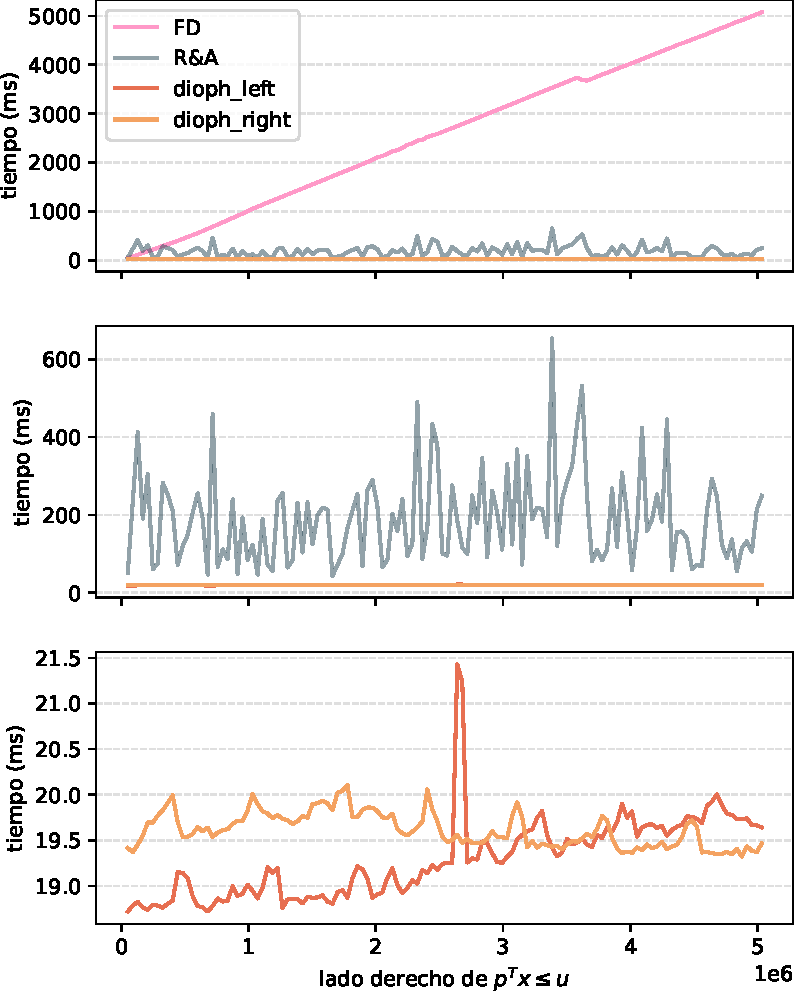
\includegraphics[width=0.9\linewidth]{/home/tempdata/repos/thesis/static/fin/rhs/times-macro.pdf}
	\caption{Tiempos de terminación promedio de los distintos métodos cuando varía el presupuesto.
		Para observar mejor los tiempos, eliminamos el método más lento y hacemos \textit{zoom} a la
		imagen.}
	\label{fig:exp:fin:rhs:zoom}
\end{figure}

\begin{figure}[hbtp]
	\centering
	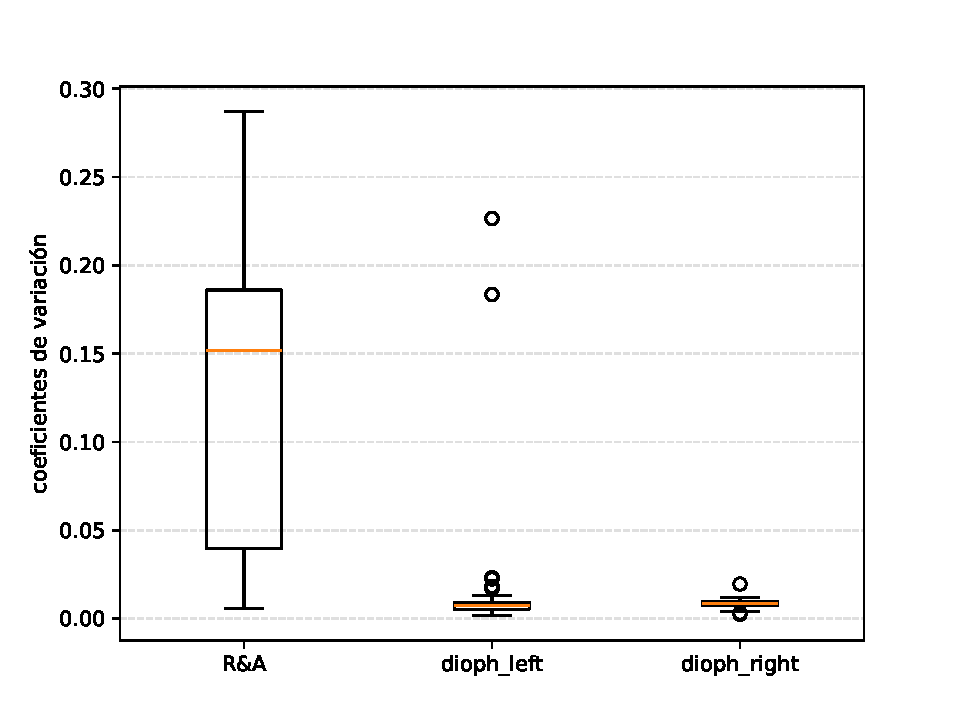
\includegraphics[width=0.9\linewidth]{/home/tempdata/repos/thesis/static/fin/rhs/boxplot-cv.pdf}
	\caption{Coeficientes de variación en los tiempos de terminación a medida que el presupuesto
	varía.}
	\label{fig:exp:fin:rhs:cv}
\end{figure}

Como mostramos en la subsección \ref{subsec:fin:dp}, se ilustra gráficamente que los tiempos de
terminación de FD crecen linealmente con respecto al presupuesto. Aún así, destaca el hecho de que
FD resultó ser más consistente en sus tiempos de terminación que los otros tres métodos. Ambos FD y
\texttt{dioph\_right} tuvieron coeficientes de variación menor que 2.5\%, al igual que
\texttt{dioph\_left} con excepción de dos experimentos anómalos.

En ambos R\&A y los métodos diofantinos hay presencia de un comportamiento oscilatorio. El autor
confirmó para los métodos diofantinos que esto coincide en la mayoría de los casos cuando el
presupuesto $u$ es múltiplo de una de las entradas de $\vec{q}$. En estos casos el problema es
trivial, pues si $q_j \mid u$, entonces uno de \texttt{dioph\_left} o \texttt{dioph\_right}
encuentra inmediatamente la solución $\vec{x} = \floor{u/q_j}\vec{e}_j$.

En los casos que una entrada de $\vec{q}$ divide a $u$, el autor encontró que un repunte en
\texttt{dioph\_left} coincide con una caída en \texttt{dioph\_right} y viceversa. Las excepciones
más notables a este comportamiento fueron las dos observaciones anómalas en \texttt{dioph\_left}
(ver figuras \ref{fig:exp:fin:rhs:zoom} y \ref{fig:exp:fin:rhs:cv}). En cambio, el comportamiento
oscilatorio en R\&A no coincide con los casos en los que el presupuesto $u$ es múltiplo de alguna
entrada de $\vec{p}$.

Destaca la inestabilidad del método de R\&A. El autor hipotetizó que esto se debe a la constante
sobrecarga computacional de transferir datos entre los módulos del problema relajado y la generación
de cortes (ver figura \ref{p1c11:fig:MIP_solver_flowchart}) dentro del \textit{solver} CBC. Por
ello, el autor decidió correr el mismo experimento tomando en cuenta una configuración de R\&A que
prohíba la generación de cortes. Debido a la dimensión $n = 1{,}000$ del problema y al fenómeno
expuesto en la sección \ref{sec:inf:exp}, no prohibimos el uso de heurísticas.

El autor encontró que los tiempos de terminación son similares y por lo tanto no tiene sentido
mostrarlos, pero sí hay un cambio significativo en la estabilidad de esta nueva configuración. La
comparación de coeficientes de variación se muestra en la figura \ref{fig:exp:fin:rhs:cv-wbb}.

Es claro que la mediana de los coeficientes de variación es aproximadamente un tercio en la
implementación sin cortes. Es decir, en el 50\% de los $N = 128$ experimentos que realizamos, las
distribuciones de los tiempos de terminación están tres veces más concentradas alrededor de su media
en la configuración sin cortes que en la configuración original. Aún así, el rango de ambas
distribuciones es la misma, lo que sugiere que en ningún momento la generación de cortes ayudó a
encontrar más rápidamente las soluciones óptimas. En realidad, la generación de cortes provocó que
Ramificación y Acotamiento se comportara erráticamente.

En conclusión, el autor considera que el argumento a favor del uso de métodos diofantinos es fuerte.
Mostramos en ambos experimentos de esta sección que los métodos diofantinos son más rápidos, más
estables y significativamente más robustos ante cambios en la dimensión o en el presupuesto del
problema \eqref{theory:formulation} que sus contrapartes FD o R\&A. El siguiente capítulo propone
una extensión de estos métodos diofantinos para resolver programas lineales enteros generales.

\begin{figure}[hbtp]
	\centering
	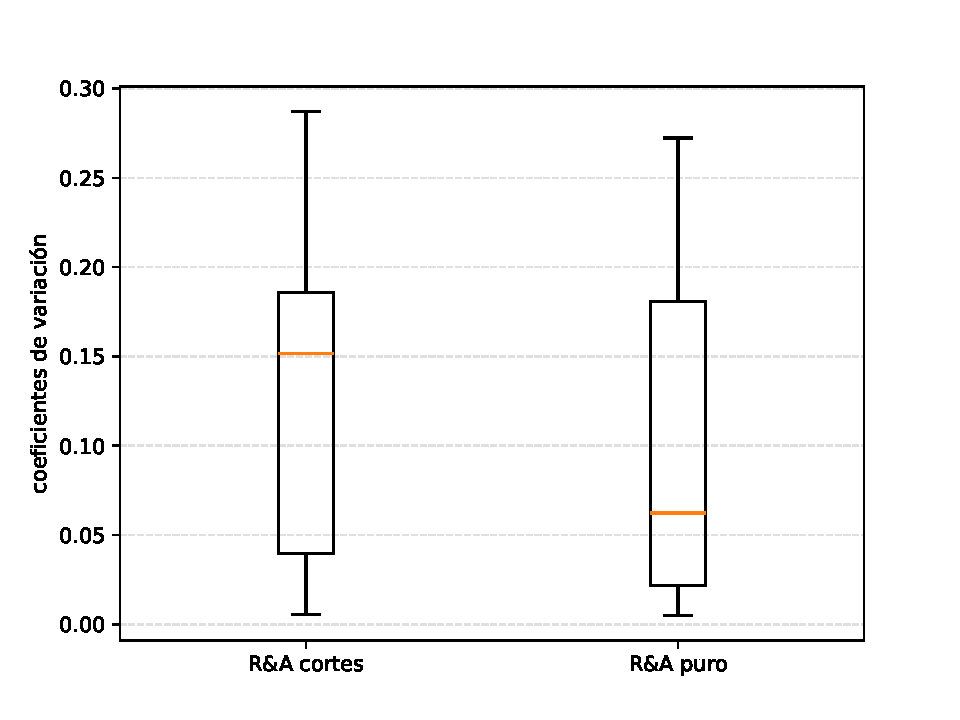
\includegraphics[width=0.9\linewidth]{/home/tempdata/repos/thesis/static/fin/rhs/boxplot-cv-wbb.pdf}
	\caption{Comparación en la estabilidad de Ramificación y Acotamiento al prohibir la generación
		de cualquier tipo de corte.}
	\label{fig:exp:fin:rhs:cv-wbb}
\end{figure}
